\documentclass{article}

% if you need to pass options to natbib, use, e.g.:
%     \PassOptionsToPackage{numbers, compress}{natbib}
% before loading neurips_2024
% ready for submission
% \usepackage[main, final]{neurips_2026}
\usepackage[main,final]{neurips_2026}
% to compile a preprint version, e.g., for submission to arXiv, add add the
% [preprint] option:
%     \usepackage[preprint]{neurips_2024}

% to compile a camera-ready version, add the [final] option, e.g.:
%     \usepackage[final]{neurips_2024}
% to avoid loading the natbib package, add option nonatbib:
%    \usepackage[nonatbib]{neurips_2024}


\usepackage[utf8]{inputenc} % allow utf-8 input
\usepackage[T1]{fontenc}    % use 8-bit T1 fonts
\usepackage{hyperref}       % hyperlinks
\usepackage{url}            % simple URL typesetting
\usepackage{booktabs}       % professional-quality tables
\usepackage{amsfonts}       % blackboard math symbols
\usepackage{nicefrac}       % compact symbols for 1/2, etc.
\usepackage{microtype}      % microtypography
\usepackage{xcolor}         % colors

%% --- our preambles --------------

%% --- packages from Wenyu's latex file
\usepackage{bbm}
\usepackage{natbib}
\setcitestyle{numbers,square}
\usepackage{tikz}
\usetikzlibrary{arrows.meta, positioning}
%% --- Wenyu's Packages end here.
\usepackage{amsmath}
\usepackage{amsthm,amsfonts}
\usepackage{graphicx}
\usepackage{autobreak}
\usepackage{diagbox}

% --- 
% \usepackage{geometry}
\usepackage{algorithm}
\usepackage{algpseudocode}
% \usepackage{fdsymbol}
\usepackage{float} 
% \usepackage{subfig} 
%\usepackage{cite}    % --- need natbib
%\usepackage[apaciteclassic]{apacite}
% \usepackage{listings}
% \usepackage{setspace}
% \usepackage{cancel}
\usepackage{mathrsfs,color}
% \usepackage[normalem]{ulem}
\usepackage{cleveref}
\usepackage{booktabs}
\graphicspath{ {Figures/} }
%\doublespacing
%\geometry{a4paper,scale=0.8}
\newtheorem{definition}{Definition}
\newtheorem{theorem}{Theorem}
\newtheorem{lemma}[theorem]{Lemma}    % lemma --> proposition

% I change prop to lemma

\newtheorem{corollary}[theorem]{Corollary}
\theoremstyle{definition}
\newtheorem{remark}{Remark}
\newtheorem{assumption}{Assumption}
\newtheorem{prop}[theorem]{Proposition}

\newtheorem{Atheorem}[theorem]{Theorem}
\newtheorem{Alemma}[theorem]{Proposition}
\newtheorem{Acorollary}[theorem]{Corollary}
\newtheorem{Aprop}[theorem]{Proposition}

\crefname{theorem}{Theorem}{Theorems}
\crefname{lemma}{Lemma}{Lemmas}
\crefname{corollary}{Corollary}{Corollaries}
\crefname{assumption}{Assumption}{Assumptions}
\crefname{prop}{Proposition}{Propositions}

\Crefname{theorem}{Theorem}{Theorems}
\Crefname{lemma}{Lemma}{Lemmas}
\Crefname{corollary}{Corollary}{Corollaries}
\Crefname{assumption}{Assumption}{Assumptions}
\Crefname{prop}{Proposition}{Propositions}

\newcommand{\cit}{\textbf{(need citation)}}

\newcommand{\CC}{\mathcal{C}}
\newcommand{\DD}{\mathcal{D}}
\newcommand{\EE}{\mathcal{E}}
\newcommand{\LL}{\mathcal{L}}
\newcommand{\UU}{\mathcal{U}}
\newcommand{\R}{\mathbb{R}}
\newcommand{\C}{\mathbb{C}}
\newcommand{\N}{\mathbb{N}}
\newcommand{\eps}{\varepsilon}
\newcommand{\om}{\omega}
\newcommand{\de}{\Delta(\eps)}
\newcommand{\ue}{u_{\alpha}(\eps}
\newcommand{\bsob}{\mathrm{H}_0}
\newcommand{\sob}{\mathrm{H}}
\newcommand{\Sa}{\mathrm{Sa}}
%\newcommand{\Sa}{\mathrm{S}}
\newcommand{\spec}{\mathrm{spec}}
\newcommand{\wenyu}[1]{\textcolor{blue}{ #1}}
%\newcommand{\wenyu}[1]{\textcolor{blue}{}}
% MMP commands
\newcommand{\mmp}[1]{\textcolor{red}{ #1}}
%\renewcommand{\mmp}[1]{}
\newcommand{\MM}{\mathcal{M}}
\newcommand{\XX}{\mathcal{X}}
\newcommand{\tilXX}{\tilde{\mathcal{X}}}
\newcommand{\tiln}{\tilde{n}}

\newcommand{\rrr}{\mathbb{R}}

\newcommand{\grad}{\operatorname{grad}}
%\newcommand{\div}{\operatorname{div}}
\newcommand{\wfs}{{\rm wfs}}

\makeatletter
\newcommand{\rmnum}[1]{\romannumeral #1}
\newcommand{\Rmnum}[1]{\expandafter\@slowromancap\romannumeral #1@}
\makeatother  

%***************** end preamble ***********************

\title{How well behaved is finite dimensional Diffusion Maps embedding?}
% Using \And between authors leaves it to LaTeX to determine where to break the
% lines. Using \AND forces a line break at that point. So, if LaTeX puts 3 of 4
% authors names on the first line, and the last on the second line, try using
% \AND instead of \And before the third author name.

\author{%
  Wenyu Bo \\
    Cheriton School of Computer Science\\
    University of Waterloo\\
    Waterloo, ON \\
    \texttt{w3bo@uwaterloo.ca} \\
  \And
  Marina Meil\u{a}  \\
  Cheriton School of Computer Science\\
    University of Waterloo\\
    Waterloo, ON \\
  \texttt{mmp@uwaterloo.ca}
   % \AND for new line
}

\begin{document}   %-------******************----------------------------


\maketitle

\begin{abstract}
  	Diffusion Maps (DM) is a well studied and popular non-linear dimension reduction algorithm. Surprisingly, while the convergence properties of DM are well understood, the {\em geometric} properties of the embedding, such as reach and smoothness have not yet been studied. Under a set of standard assumptions on a family of submanifolds $\subset \R^D$, we derive a series of geometric properties that are preserved by DM, including almost uniform density, finite polynomial approximation and reach. Leveraging these properties, we establish rigorous bounds on the embedding errors introduced by the DM algorithm, of the order $(\frac{\log n}{n})^{\frac{1}{8d+16}}$. 
    \iffalse
    Furthermore, by using a subsampling setting, we quantify the error between the estimated tangent spaces and the true tangent spaces over the submanifolds after the DM embedding to be $\sim(\frac{\log n }{n})^\frac{k-1}{(8d+16)k}$,  providing a precise characterization of the geometric accuracy of the embeddings. 
    \fi
    These results offer a solid theoretical foundation for understanding the performance and reliability of DM in practical applications.
\end{abstract}


\section{Introduction}
\label{nips:sec:intro}
\iffalse
DM \cite{COIFMAN20065,coifman2008diffusion}(coifman-lafon and the others) revolutionized/marked a turning point int non-linear dimension reduction, both wrt its theoretical understanding and its practical applicability. DM is now widely used in scientific data analysis \mmp{cite as many papers as we can} and is arguably the most studied dimension reduction method \mmp{cite as many as we can}. It also engendered a novel work in dimension reduction \cite{} and resurfaced/ XXXX traditional work \cite{}.

We now know that \mmp{again cite as many as we can, with facts}

This paper builds on the above body of knowledge to consider the following high level questions/distilling from it a ``profile'' for the DM embedding and its properties. 


ORIGINAL NEURIPS INTRO
\fi
Low dimensional embeddings of high-dimensional data are often used for visualization \cite{tsne}, i.e. as the {\em last step} of a data analysis. We ask whether non-linear dimension reduction, performed in a principled way, can also be useful as a {\em first step} of the data analysis, just like the classical Principal Component Analysis. Therefore, this paper examines to what extent the Diffusion Maps (DM) embedding\cite{COIFMAN20065,belkin2003laplacian}, a dimensionality reduction technique that captures the geometric structure of data by constructing a diffusion process among data points, obtains ``well conditioned'' non-linear embeddings, i.e. embeddings whose geometric distortions can be bounded.

Of particular interest is the preservation of the tangent space estimation under the DM embedding. For a smooth function on a manifold $M$, its gradient (as well as higher order derivatives) live in the tangent space to $M$. Controlling the error of the tangent space estimation in finite sample settings is a necessary condition to ensure that the gradients of functions of interest are transported unbiasedly to the lower dimensional data representation.

The DM is well studied as a differential geometric object; \cite{berard1994embedding} showed that in the limit of infinite dimension it is an isometric embedding, while \cite{portegies2016embeddings} showed that almost isometry can be achieved with a finite number $m$ of eigenfunctions, where this $m$ depends on manifold geometric properties. \cite{bates2014embedding} showed that if isometry is not required, then the sufficient embedding dimension by Laplacian eigenfunctions depends on dimension, injectivity radius, Ricci curvature and volume, thus that it can be arbitrarily larger than the Whitney embedding dimension of $2d$.

The DM embedding is widely used for non-linear dimension reduction as the Diffusion Maps algorithm \cite{COIFMAN20065,lafon2006diffusion,coifman2008diffusion,arvizu2016dimensionality}, which embeds a sample into $m$ dimensions by the eigenvectors of $L_n$, a $n\times n$ matrix estimator of the Laplace-Beltrami operator $\Delta$.
For instance, DM was used to analyze high-dimensional single-cell RNA sequencing data, revealing cell differentiation trajectories and underlying biological patterns\cite{haghverdi2015diffusion}, and it can order cells along their differentiation paths, enabling accurate reconstruction of branching developmental processes\cite{haghverdi2016diffusion}. 
In chemistry, DM can extract the dynamical modes of high-dimensional simulation trajectories, furnishing a kinetically low-dimensional framework\cite{ferguson2011nonlinear}, it can identify the collective coordinates of rare events in molecular transitions\cite{boninsegna2015investigating}.
In Astronomy, DM is applied to estimate galaxy redshifts from photometric data, demonstrating comparable accuracy to existing methods\cite{freeman2009photometric}.

Stimulated in part by the practical applications of DM, the consistency of  finite sample estimators of $\Delta$, and of their eigenfunctions has been intensely studied. Many early works discussed the pointwise consistency for empirical operator with smooth functions on $M$ and they derived convergence (with different rates) \cite{von2008consistency,belkin2008towards,gine2006empirical,10.5555/3104322.3104459,hein2007graph}, which provide illuminating results for subsequent studies. Not only $\Delta$ itself, the consistency of its embedding are also widely studied, they discussed how the eigenvectors and eigenvalues of the empirical Laplacian with specific graph (K-NN, $\epsilon$-graph) converge to the eigenfunctions and eigenvalues of $\Delta$ in the different norm ($L^2$, $L^\infty$)\cite{cheng2022eigen,garcia2020error,wang2015spectral,belkin2006convergence}. There are some other special convergence types studied. For instance, convergence in Lipschitz norm\cite{calder2022lipschitz}, embedding using heat kernel\cite{jones2008manifold,DUNSON2021282}

This paper completes the picture by considering geometric properties of a manifold, such as smoothness, injectivity radius, reach, volume, diameter, and examining to what extent the DM preserves these properties. In other words, if the original manifold $\MM$ is ``well behaved'', what can be said about its DM embedding $\varphi(\MM)$? Surprisingly, these questions have received less attention in the literature.

Specifically, under a set of mostly standard geometric assumptions on a family of compact manifolds (\cref{sec:problem}), in \cref{sec:phim-L} we study the smoothness of $\varphi$ by examining its Sobolev norms (\cref{sec:smooth}) and use it to show the existence of local parameterizations, then we derived consistent properties that hold uniformly for all manifolds in the family after DM embedding, like sampling densities and reach (\cref{phiM}). In \cref{sec:convergence}, we identify the correspondence between the embedding via eigenfunctions and the embedding via eigenvectors of the graph matrix and address the convergence between them, then estimate the error between the eigenfunctions and eigenvectors to quantify the noise in the positions of the embedded points. \cref{sec:experiments} presents the experimental results, and \cref{sec:conclusion} concludes the paper.

 
\section{Background, challenges and assumptions}
\label{sec:problem}

\subsection{Manifolds and geometric preliminaries}
For basic definitions readers should consult \cite{do1992riemannian,lee2003introduction,lee2018introduction}. Here we consider sub-manifolds $M\subset \rrr^D$ which we will generically call {\em manifolds}. Note that the ambient dimension $D$ will not appear throughout the paper, only Euclidean distances $|x-y|$ with $x,y\in \rrr^D$ will appear, hence $D$ can actually be infinite, and $\rrr^D$ could become a Hilbert space.

We also assume that $M$ is a closed manifold with smoothness of class $\mathcal{C}^k$, as described in \cref{as:smooth}. This assumption ensures the existence of a local polynomial expansion up to order $k$ in the neighborhood of each point on $M$. Such expansions satisfy specific regularity constraints, enabling precise characterization of the local geometry and supporting rigorous analytical derivations. These properties are fundamental for establishing the theoretical results and ensuring consistency in subsequent computations.

In this work, we focus on several key geometric quantities, including the tangent space, reach, Riemannian metric, and geodesic curves. These quantities play critical roles in understanding the geometry of the manifold and in estimating and reconstructing manifolds. While these concepts are broadly defined in the general framework in Riemannian geometry, considering that our sampling points lie in submanifolds of $\R^D$, we restrict our attention to their specialized formulations for submanifolds embedded in Euclidean space. This setting simplifies their definitions and aligns with the analytical and computational techniques employed in this study. For example, the tangent space is characterized as the hyperplane tangent to $M$ at a given point, and the Riemannian metric is induced from the ambient Euclidean metric. 

For definition of \textbf{Tangent Space}, \textbf{Riemannian Metric}, \textbf{Normal Coordinate} and \textbf{Laplace-Beltrami Operator}, please refer to \cite{lee2018introduction}. We will talk about other geometric quantities in the following.

Riemannian metric defines a measure on $M$, called the {\em Riemannian measure} via the {\em volume form}. If $M$ is compact, it has a finite volume $\text{Vol}(M)$. We can now have other measures on $M$, which are absolutely continuous w.r.t. the Riemannian measure, through their densities $f:M\rightarrow (0,\infty)$.   In statistics/manifold learning, it is assumed that we are given an i.i.d. sample $X_n=\{x_1,\ldots x_n\}\subset M$ from $f$. 


\begin{definition}[Reach\cite{federer1959curvature}]
	\upshape
	The reach of a subset $A$ of $\R^n$ is the largest $\tau$ (possibly $\infty$) such that if $x \in\R^n$ and the  distance from $x$ to $A$ is smaller than $\tau$, then $A$ contains a unique point nearest to $x$. For more detail and properties, refer to \cite{aamari2019estimating}.
\end{definition}
The reach of a subset $A \subset \R^n$  provides a measure of its local geometric regularity. Specifically, if the reach of  $A$ is $\tau>0$, then every point within a distance less than $\tau$ from $A$ has a unique nearest point on $A$. Geometrically, this implies that $A$ does not exhibit sharp corners, cusps, or regions of high curvature within the specified radius. In particular: For convex subsets of $\R^n$, the reach is infinite, reflecting the absence of curvature bounds or sharp features. For smooth submanifolds, the reach is inversely related to its maximum principal curvature. Intuitively, the reach corresponds to the radius of the smallest osculating ball that fits locally around.




\subsection{The Diffusion map}
\label{embed}
Let $M$ be a smooth, closed manifold of class $\mathcal{C}^3$ embedded in the (possibly high-dimensional) Euclidean space $\rrr^D$ and $\Delta_{\mathcal{M}}$ be Laplacian operator on $M$ with eigenvalues $0=\lambda_0 \leq \lambda_1 \leq \cdots$. We consider eigenfunctions corresponding to these eigenvalues: $e_0,e_1,\cdots$, and we normalize them such that $\|e_i\|_{L^2}=1$. It is easy to check $e_0 \equiv \mathrm{const}$. Then we have the following embedding theorem.


\begin{theorem}\cite[Thm. 5.1]{portegies2016embeddings}
	\label{embeddingthm}
Let $\MM$ be the set of $d$ dimensional, closed Riemannian manifolds whose Ricci curvature is bounded from below by $\kappa$, injectivity radius is bounded from below by $\iota$, and the volume is bounded from above by $V$, we define $\varphi: M\subset \mathbb{R}^D \rightarrow \varphi(M) \subset \mathbb{R}^m$ as the following:
\begin{equation}
	\varphi(x)=(2t)^\frac{d+2}{4}\sqrt{2}(4\pi)^\frac{d}{4}(e^{-\lambda_1 t}e_1(x),e^{-\lambda_2 t}e_2(x),\cdots,e^{-\lambda_m t}e_m(x)) \in \mathbb{R}^m,
\end{equation}
then there exists a $t_0=t_0(d,\kappa,\iota,\epsilon)$ such that for all $0<t<t_0$, there exists a $N_0(d,\kappa,\iota,\epsilon,V,t)$ such that if $m>N_0$, then for all $M\in \mathcal{M}(d,\kappa,\iota,V)$, the map above is an embedding of $M$ into $\mathbb{R}^m$, and $1-\epsilon < \|d \varphi_p v\| < 1+\epsilon$ where $\|v\|=1$.
\end{theorem}


\begin{lemma}\cite[Lem. 3.2]{portegies2016embeddings}
	\label{kernelerror}
We use the same notation as in the preceding theorem. Then for $\epsilon^\prime>0$, there exists $N_1=N_1(d,\kappa,\iota,V,\epsilon^\prime,t_0)$ such that when $m\geq N_1$ and $t_0 \leq t^\prime\leq 4$, we have 
\begin{align}
	\left|K_m(t^\prime,p,\cdot)-K(t^\prime,p,\cdot)\right| \leq \epsilon^\prime,
\end{align}
where $K(t,p,q)$ is the heat kernel:
$K(t,p,q)=\sum_{i=0}^{\infty} e^{-\lambda_i t} e_i(p) e_i(q)$,
and $K_m(t,p,q)$ is the truncated heat kernel:
$K_m(t,p,q)=\sum_{i=0}^{m} e^{-\lambda_i t} e_i(p) e_i(q)$. 
\end{lemma}

We select $t=t_0/2$, $t^\prime = t_0$ (if $t_0>4$, we set $t=2$ and $t^\prime=4$) and $m=\max\left\{N_0,N_1\right\}+1$ to make the results above both hold.


In addition, $\varphi:M\rightarrow \varphi(M)$ is a homeomorphism, so $\dim M=\dim \varphi(M)$, and $\varphi$ is an embedding, also an immersion, thus $\varphi$ is a local diffeomorphism, and $\varphi$ is bijective, so $\varphi$ is a diffeomorphism. Thus $\varphi(M)$ is a smooth manifold \cite{lee2003introduction}.

\iffalse

\mmp{
\begin{enumerate}
	\item We have $n$ samples $\left\{x_{1:n}\right\} \overset{i.i.d.}{\sim} M$, where $M$ is a d-dimensional manifold, and $x_i \in \mathbb{R}^D$.
	\item Using Embedding Algorithm (DM), we have $\left\{y_{1:n}\right\}=\hat{\varphi}(x_{1:n}) \in \mathbb{R}^m$ where $m\geq d$.
	\item We estimate Tangent Space $\Tilde{T_i}$, and want to estimate $\Vert Err(\Tilde{T_i}) \Vert$.
\end{enumerate}
shall we be consistent about $x\in M, \,y\in\varphi(M)$?
}%end mmp 
\fi

Given a finite sample $\mathcal{X}_n=\left\{x_1,\dots,x_n\right\}$ the DM algorithm constructs a similarity matrix to measure the pairwise relationships between data points, where the commonly used kernel is the Gaussian kernel, defined as $k(x_i, x_j) = \exp(-\|x_i - x_j\|^2 / h)$, where $h$ is a scale parameter, and this similarity matrix is then normalized, we denote it as Laplacian graph which is the approximation of Laplace-Beltrami operator. By performing eigenvalue decomposition on normalized Laplacian graph, the algorithm extracts the dominant eigenvalues and eigenvectors. These eigenvectors, scaled by their corresponding eigenvalues, define the diffusion coordinates, providing a low-dimensional embedding of the data. This embedding preserves the global geometry of the dataset while emphasizing its intrinsic structure.



In this paper, we will focus mainly on the geometric properties of the DM $\varphi(M)$, w.r.t. the original manifold $M$. The results we obtain will be useful in characterizing the output of the DM algorithm in finite sample settings.
\iffalse
and we apply them specifically to the
estimation of the tangent subspace $\left\{T_{\varphi(x_i)}\varphi(x_i)\right\}_{i=1}^n$.
\fi

\cite{berard1994embedding} have shown that, in the limit of large $m$ and small $t$, $\varphi(M)$ is isometric with $M$, and that this is possible approximatively with a finite $m$ for manifolds with bounded diameter and Ricci curvature bounded from below. In spite of these seemingly encouraging results, the DM can exhibit severe curvature distortions even for apparently ``nice'' manifolds. The intuitive explanation is the fact that, even if $M$ is compact and smooth to order $k$, the local interactions between the manifold curvature and the manifold reach (note that these are not independent quantities) can exert a strong influence on the Laplacian eigenfunctions. 

\subsection{Assumptions}

Thus, in predicting smoothness (w.r.t. Sobolev norms) and geometric properties of $\varphi(M)$, one needs to consider $\tau_M, \iota_M, \kappa_M$ in addition to the smoothness of $M$ (made more precise below). We will give the assumptions for the set of manifolds we will perform DM, and then discuss basic properties of $M$ based on these assumptions. We will see all these assumptions intuitively ensure our manifolds have very good shape, which can help us avoid extremely bizarre situations. And we will use them to derive existence of the geometric bound after DM, which are critical in estimating the convergence rate.


\begin{assumption}[Reach]
	\label{as:reach}
  The reach $\tau_M$ of $M$ is bounded below by $\tau_{\min}$. This assumption is used in \cref{thm:reach-bound}.
\end{assumption}

\begin{assumption}[Volume]
	\label{ass:V}
  The volume of $M$ is bounded below by $V_1$ and bounded above by $V_2$. This assumption is used in \cref{embeddingthm}, \cref{lem:lambdam-bound}.
\end{assumption}

\begin{assumption}[Smoothness]
	\label{as:smooth}
For $k$ and $\textbf{L}:=\left(L_\perp,L_3,\dots,L_k\right)$, we assume there exists a local one-to-one parameterization $\Psi_p$ for all $p \in M$:
	\begin{align}
		\Psi_p :B_{T_pM}(0,r) \rightarrow M \quad \text{by} \quad \Psi_p(v)=p+v+N_p(v)
	\end{align}
	for some $r\geq \frac{1}{4L_\perp}$ with $N_p(v) \in \mathcal{C}^k(B_{T_pM}(0,r),\mathbb{R}^D)$ such that 
	\begin{align}
		N_p(0)=p,\  d_0N_p=0,\ \|d_v^2N_p\| \leq L_\perp, \ \|d_v^iN_p\|\leq L_i\ \text{for }i=3,\dots,k
	\end{align}
	holds for all $\|v\|\leq \frac{1}{4L_\perp}$. This assumption is used in \cref{lem:remainder-bound}
\end{assumption}


In addition, we make the following more technical regularity
assumption that will be used in \cref{lem:covar-deri-bound}, \cref{sec:glo-reach}.


\begin{assumption}[Christoffel Symbols]
	\label{as:Christoffel}
	In the normal coordinate chart, the derivatives of the Christoffel symbols of order at most $k-2$ (including Christoffel symbol itself) have a uniform upper bound depending only on its order, i.e.
	\begin{align}
		|\frac{\partial^l \Gamma_{ij}^k}{\partial x_{i_1}\cdots\partial x_{i_l}}| \leq C(l) \quad \text{for } 1\leq i,j,k\leq d\ \text{ and }\  l\leq k-2
	\end{align}
\end{assumption}

\begin{assumption}[Heat Kernel Bound]
    \label{as:heatkernel}
    The heat kernel coefficients $\Phi_j(p,q)$ and $C(v)$ are uniformly bounded with respect to $d(p,q) \in (s_0, s_1)$. \cref{eq:heatkernelcoef}.
\end{assumption}


Let $\mathcal{M}(d,\tau_{\min},V,k,\textbf{L},\Gamma)$ be the set of compact connected submanifolds $M \subset \mathbb{R}^D$, with dimension $d$ satisfying \cref{as:reach}--\cref{as:heatkernel}. For simplicity, in the rest of our paper we always assume that the manifold is $d$-dimensional and the ambient dimension is $D$, we also use the abbreviation $\mathcal{M}$ for $\mathcal{M}(d,\tau_{\min},V,k,\textbf{L},\Gamma)$, and sometimes we include some of the parameters above to indicate that the assumptions corresponding to these parameters are satisfied.


We also assume that the sampling density on $M$ does not deviate too much from uniform.
\begin{assumption}[Density]
\label{ass:density}
  Let $\mathcal{P}_{f_{\min},f_{\max}}$ denote the set of distributions $P$ with support on $M \in \mathcal{M}$, and the density function $f$ of $P$ with respect to Hausdorff measure such that $0<f_{\min}\leq f \leq f_{\max}<\infty$. This assumption will be used in \cref{sec:density}.
\end{assumption}

All the assumptions above, perhaps with the exception of \cref{as:smooth}, \cref{as:Christoffel}, and \cref{as:heatkernel} are generically present in the manifold learning literature.


\subsection{Direct Consequences of Assumptions}
Here we list some direct results for $M \in \MM$ from assumptions which will also be used in our following proof.

\begin{corollary}[Complete Manifold]\cite{do1992riemannian}
	Any compact Riemannian manifold is geodesically complete according to the Hopf-Rinow theorem.
\end{corollary}

\begin{corollary}[Curvature]
	\label[corollary]{as:kappa}
	The sectional curvature of $M$ is bounded by $\kappa$, since $|K(u,v)|\leq 2/\tau_M^2 \leq 2 / \tau_{\min}^2$ due to the Gauss equation. In addition, it immediately implies Ricci curvature of $M$ is bounded below by $-\kappa(d-1)$ since $\operatorname{Ric}(v,v)=\sum_{i=2}^{d}K(v,x_i)$ where $\left\{v, x_2,\dots,x_d\right\}$ are orthonormal basis. It is used in \cref{embeddingthm}, \cref{lem:lambdam-bound}.	
\end{corollary}

\begin{corollary}[The injectivity radius]\cite[Prop. A.1]{aamari2019estimating}
	\label[corollary]{injradius}
	The injectivity radius $\iota_M$ of $M$ is bounded below by $ \pi \tau_M$, which implies $\iota_M$ is bounded by $\pi \tau_{\min}$ for all $M \in \MM$. We use it to make sure DM is an embedding.
\end{corollary}
The injectivity radius bounded from below implies we can find a normal coordinate chart with the uniform radius.

\begin{corollary}[Diameter]\cite[Lem. 2]{aamari2018stability}
	For $M \in \mathcal{M}$, we have
	\begin{align}
		\operatorname{diam}(M)\leq \frac{C_d}{\tau_M^{d-1}f_{\min}}\leq \frac{C_d}{\tau_{\min}^{d-1}f_{\min}}
	\end{align}
	where $C_d$ is a constant only depending on $d$. Thus the diameter of $M \in \mathcal{M}$ has a uniform upper bound. We will use it in \cref{lem:lambdam-bound}.
\end{corollary}


   % dm-arxiv-assumptions.tex merged here
\section{Properties of the diffusion maps embedding \texorpdfstring{$\varphi(\mathcal{M})$}{phi(M)}}
\label{sec:phiM-summary}
In this section, we will discuss the properties of $\varphi(M)$, here we collect  the uniform estimates for the family $\varphi(\MM)$ and make explicit the logical chain that connects them. We will prove that the family $\varphi(\mathcal{M}) \in \mathcal{M}(\tau_{\varphi(M)},\textbf{L}^\prime)$ where $\textbf{L}^\prime:=\left(L_\perp^\prime,\dots,L_k^\prime\right)$ and the density function of $\varphi(M)\in  \varphi(\mathcal{M})$ admits uniform upper and lower bounds.
The proofs are presented in full in \cref{phiM}; here we only state the results and indicate the logical chain.

The dependency chain is
\begin{center}
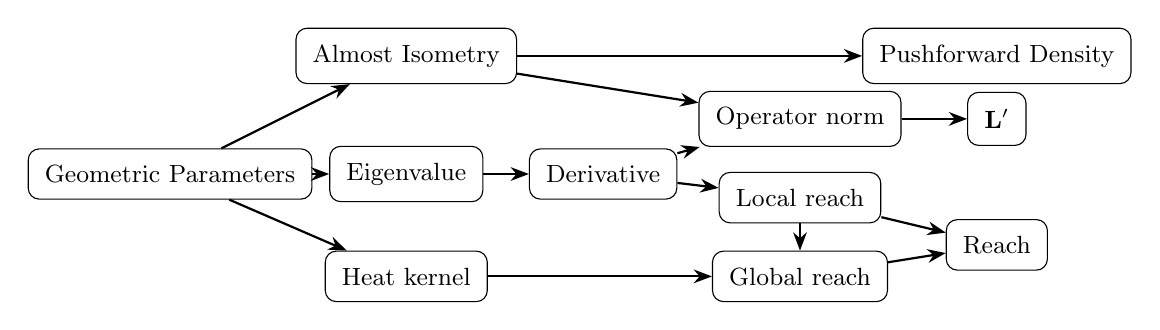
\begin{tikzpicture}[
    >=Stealth,
    node distance=1.1cm and 1.5cm,
    every node/.style={
        draw,
        rounded corners,
        align=center,
        font=\small,
        inner sep=6pt
    },
    arr/.style={->, thick}
]
    % Main nodes
	\node (par) at (-3, 0.5) {Geometric Parameters};
    \node (iso) at (0, 2) {Almost Isometry};
    \node (eig) at (0, 0.5) {Eigenvalue};
    \node (der) at (2.5, 0.5) {Derivative};
    \node (norm) at (5, 1.2) {Operator norm};
    \node (L) at (7.5, 1.2) {$\textbf{L}^\prime$};

    % Reach-related nodes
    \node (heat) at (0, -0.8) {Heat kernel};
    \node (local) at (5, 0.2) {Local reach};
    \node (global) at (5, -0.8) {Global reach};
    \node (reach) at (7.5, -0.4) {Reach};

    % Density
    \node (density) at (7.5, 2) {Pushforward Density};

    % Arrows

	\draw[arr] (par) -- (iso);
	\draw[arr] (par) -- (eig);
	\draw[arr] (par) -- (heat);

    \draw[arr] (iso) -- (density);
    \draw[arr] (iso) -- (norm);

    \draw[arr] (eig) -- (der);
    \draw[arr] (der) -- (norm);
    \draw[arr] (norm) -- (L);

    \draw[arr] (der) -- (local);

    \draw[arr] (heat) -- (global);
    \draw[arr] (local) -- (global);
    \draw[arr] (local) -- (reach);
    \draw[arr] (global) -- (reach);
\end{tikzpicture}
\end{center}

To begin with, we establish the uniform upper bound on the eigenvalues.
Using the Li--Yau estimates \cite[Thm. 16]{esteigenvalue}, the Laplacian eigenvalues grow at a controlled rate uniformly over the family $\MM$.

\textbf{\cref{lem:lambdam-bound}.} 	There exists a constant $C$ depending only on the uniform geometric parameters $(d,\kappa,\mathrm{diam},V)$ of the family $\MM$, such that
	\begin{align}
		\lambda_k \leq C (k+1)^\frac{2}{d} \qquad \text{for all } M \in \MM.
	\end{align}
We next derive uniform bounds on the eigenfunction derivatives.
Using the eigenvalue estimate in Step~1, together with estimates in \cite{2004Xuhigherorder}, we can control the derivatives of the eigenfunctions, and the coordinate derivatives of each component of $\varphi$.

\textbf{\cref{lem:eigfn-deri-bound}.} 
For every multi--index $\alpha$ with $|\alpha| \leq k$, there exists a constant $C_\alpha$ depending only on $\alpha$ and the uniform geometric parameters of $\MM$, such that
	\begin{align}
		|\partial^\alpha e_\lambda(x)| \leq C_\alpha (1+\lambda)^{k/2+d/4}, \qquad |\alpha| \leq k.
	\end{align}
Consequently, since $\lambda_k$ is bounded above by $C(\MM)(k+1)^\frac{2}{d}$, $\varphi_j = (2t)^\frac{d+2}{4}\sqrt{2}(4\pi)^\frac{d}{4}e^{-\lambda_1 t}e_j(x)$, then the coordinate derivatives of $\varphi$ up to order $k$ are uniformly bounded over $M \in \MM$.


With the bound on the eigenfunction derivatives, we turn to the uniform bound on the operator norm of $d^l\varphi$.
Computing coordinate representation for the covariant derivatives and pluging in the bound from Step~2 with the bound of Christoffel symbols, we obtain the bound on the operator norm of $d^l \varphi$.

\textbf{\cref{lem:covar-deri-bound}.} 
For every $l \leq k$, there exists a constant $A(l)$, depending only on $l$ and the uniform geometric parameters of $\MM$, such that
	\begin{align}
		\|d^l \varphi\| \leq \sqrt{m}\,A(l)\,d^{l/2} \quad \text{for all } M \in \MM.
	\end{align}

We next control the parametrization remainder uniformly.
Expanding the remainder of the local parametrization of $\varphi(M)$ through
Fa\`a di Bruno's formula, each term is a composition of derivatives of $\varphi$
(bounded in Step~3), derivatives of the original remainder $\Psi_p$ (bounded
by Assumption~\ref{as:smooth}), and derivative of the inverse of $\varphi$ (bounded due to embedding is almost isometric), hence obtaining a parameter vector $\textbf{L}^\prime:=\left(L_\perp^\prime,\dots,L_k^\prime\right)$ controlling the remainder over $\varphi(\MM)$.
	
\textbf{\cref{lem:remainder-bound}.} There exists $\textbf{L}^\prime:=\left(L_\perp^\prime,\dots,L_k^\prime\right)$ depending only on the uniform geometric parameters of $\MM$, such that for every $M \in \MM$ and every $p^\prime=\varphi(p)$, the remainder satisfies \begin{align}
N^\prime_{p^\prime}(0)=0, d_0 N^\prime_{p^\prime}=0, \text{ and } \|d^l_{v^\prime} N^\prime_{p^\prime}\| \leq L_l^\prime \text{ for } 2 \leq l \leq k.
\end{align}


We then establish the uniform bound on the pushforward density.
Since $\varphi$ is almost isometric ($|\,\|d\varphi\|-1|<\epsilon$), the Jacobian factor stays close to $1$, so the pushforward sampling density $g$ of $\varphi_\# P$ stays comparable to the original density $f$ of the distribution $P$.

\textbf{\cref{lem:density-bound}.} 
Suppose $\epsilon \leq \frac{1-4^{-1/d}}{3}$, then for every $M \in \MM$ the Jacobian factor of $\varphi$ lies in $(\tfrac12,2)$, and consequently the pushforward density $g$ of $\varphi_\# P$ obeys $\tfrac{f_{\min}}{2} < g < 2 f_{\max}$. 


Finally, we derive a uniform lower bound on the reach.
Writing $\tau = \min\{\tau_l,\tau_g\}$, we bound the local and global reach separately.
The local reach is controlled through the second fundamental form of $\varphi(M)$,
whose operator norm is estimated directly from the second-order eigenfunction
derivative.

\textbf{\cref{lem:local-reach} (Local reach).} There exists a constant $\tau_{l,\varphi(\MM)}>0$, depending only on the uniform geometric parameters of $\MM$ and on $(m,t_0)$, such that
	\begin{align}
		\tau_{l,\varphi(M)} \geq \tau_{l,\varphi(\MM)} >0, \quad \text{for all $\varphi(M) \in \varphi(\MM)$.}
	\end{align}

For the global reach, we split the proof according to three ranges of the geodesic distance $d(p,q)$, with $s_0 = 2\sqrt{2}\,\tau_{l,\varphi(M)}$ and a threshold $s_1$:
\begin{enumerate}
	\item[(i)] $d(p,q) \leq s_0/(1+\epsilon)$. We get $d(\varphi(p),\varphi(q)) \leq s_0$ since $\varphi$ is almost isometric, and by local linear approximation (\cref{lem:geodis_eucdis,lem:global_case}) shows $\varphi(p),\varphi(q)$ cannot form a bottleneck.
	\item[(ii)] $d(p,q) > s_1$. Heat-kernel estimates give the global reach condition $|\varphi(p)-\varphi(q)| > r_1 > 0$ (\cref{global condition}).
	\item[(iii)] $s_0/(1+\epsilon) < d(p,q) < s_1$. It is empty whenever $(*)$ holds, where (i) and (ii) already cover all cases. If $(*)$ fails, we verify $d(p,q)$ in this interval. We use a tighter lower bound on $s_0$, and a short time expansion of the heat kernel that controls $K(t,p,p)-K(t,p,q)$.
\end{enumerate}
Since the three ranges cover all $d(p,q) > 0$, the global reach of $\varphi(M)$ is bounded below by a positive constant uniformly over $\varphi(\MM)$. Together, the local and global bounds give the reach theorem.

\textbf{\cref{thm:reach-bound}.} There exists a positive constant $\tau_{\varphi(\MM)}$, depending only on the uniform geometric parameters of $\MM$ and on $(m,t_0)$, such that $\tau_{\varphi(M)} \geq \tau_{\varphi(\MM)} > 0$ for all $M \in \MM$.



\section{Finite sample error of Diffusion Map \texorpdfstring{$\varphi$}{phi}}
        \label{sec:convergence}

In this section, we consider the finite-sample DM. We use a result from \cite{DUNSON2021282} to derive an $l_\infty$ simultaneous convergence rate for the DM embedding of the sample points $\mathcal{X}_n=\left\{x_1,\dots,x_n\right\}\subset M \in \mathcal{M}$. This uniform bound shows that the finite-sample DM embedding points can be viewed as discrete samples from the differential-geometric DM embedding manifold studied in Section 3, with a vanishing approximation error. Consequently, the finite-sample DM embeddings asymptotically approximate the geometric structure of the DM embedding manifold studied in Section 3.

We consider $n$ sample points $\mathcal{X}_n=\left\{x_1,\dots,x_n\right\}\subset M \in \mathcal{M}$, we define graph affinity matrix $W$ and the degree matrix $D$ as $W_{ij}=\frac{k_h (x_i,x_j)}{q_h(x_i)q_h(x_j)}, D_{ii}=\sum_{j=1}^n W_{ij}$,
where $k_h(x,y)=\exp \left(-\frac{|x-y|^2}{4h^2}\right)$ is the Gaussian kernel and $q_h(x)=\sum_{i=1}^n k_h(x,x_i)$. Then the normalized graph Laplacian $L_n$ is defined as 
\begin{align}
\label{Lap matrix}
L_n=\frac{D^{-1}W-I}{h^2}.
\end{align}

We denote the $i$-th eigenvalue of $-L_n$ as $\mu_{i,n,h}$ with corresponding eigenvector $\tilde{v}_{i,n,h}$ normalized in $l^2$ norm. It is easy to verify that $\mu_{0,n,h}=0$ and $\tilde{v}_{0,n,h} = \mathbbm{1}$. Let $\mathbb{N}(i)=|B_h(x_i) \cap \left\{x_1,\dots,x_n\right\}|$ which is the cardinality of points in the $h$-ball of $x_i$. Then we define the $l^2$ norm of $\tilde{v}$ with respect to inverse estimate density $1/\hat{p}$ as:
\begin{align}
	\|\tilde{v}\|_{l^2(1/\hat{p})} = \sqrt{\frac{|S^{d-1}|h^d}{d}\sum_{i=1}^{n}\frac{\tilde{v}^2(i)}{\mathbb{N}(i)}},
\end{align}
and we define $v_{i,n,h}=\frac{\tilde{v}_{i,n,h}}{\|\tilde{v}_{i,n,h}\|_{l^2(1/\hat{p})}}$.


Let $\Delta$ be the Laplace-Beltrami operator of $M$, and $0=\lambda_0<\lambda_1\leq \lambda_2 \leq \cdots$ be the eigenvalues of $-\Delta$. Let $e_i$ be the eigenfunctions of $-\Delta$ corresponding to $\lambda_i$. Then we have
\begin{theorem}  \cite[Thm. 2]{DUNSON2021282}
	\label{thm:conver_rate}
Let $M$ be a $d$-dimensional smooth, closed and connected Riemannian manifold embedded in $\R^D$, $f$ be the smooth probability density function on $M$ with infimum $f_{\min}>0$ and $\mathcal{X}_n=\left\{x_1, \dots,x_n\right\}$ be the point cloud sampled following $f$ independently and identically. Suppose eigenvalues of $\Delta$ are simple. For fixed $m\in \N$, denote $\Gamma_m=\min\limits_{1\leq i \leq m} \text{dist}(\lambda_i, \sigma(-\Delta)\backslash\left\{\lambda_i\right\})$, where $\sigma(-\Delta)$ is the spectrum of $-\Delta$. Suppose 
\begin{align}
	h \leq \mathcal{K}_1 \min \left(\left(\frac{\min(\mathsf\Gamma_m,1)}{\mathcal{K}_2+\lambda_m^{d/2+5}}\right)^2,\, \frac{1}{(\mathcal{K}_3+\lambda_m^{(5d+7)/4})^2}\right),
\end{align}
where $\mathcal{K}_1$ and $\mathcal{K}_2, \mathcal{K}_3>1$  are constants depending on $d$, $f_{\min}$, $\|f\|_{C^2}$, and the volume, the injectivity radius, the curvature and the second fundamental form of the manifold.
Then, when $n$ is sufficiently large so that $h=h(n) \geq (\frac{\log n}{n})^{\frac{1}{4d+13}}$, with probability greater than $1-n^{-2}$, for all $0 \leq i < m$, 
\begin{align}
	|\mu_{i,n,h}-\lambda_{i}|\leq \Omega_1 h^{3/2}. 
\end{align}
And when $n$ is sufficiently large so that $h=h(n)\geq (\frac{\log n}{n})^{\frac{1}{4d+8}} $, with probability greater than $1-n^{-2}$, there are $a_i \in \{1,-1\}$ such that for all $0 \leq i <  m$, 
	\begin{align}
		\max_{x_j \in \mathcal{X}_n}|a_i v_{i,n,\epsilon}(j)-e_{i}(x_j)|\leq  \Omega_2 h^{1/2}.
	\end{align}
$\Omega_1$ depends on $d$, the diameter of $M$, $f_{\min}$, $\|f\|_{C^2}$, and $\Omega_2$ depends on $d$, the diameter and the volume of $M$, $f_{\min}$, and $\|f\|_{C^2}$.
\end{theorem} 
\begin{remark}
In our setting, the sampling is uniform, thus $f \equiv 1/\text{Vol}(M)$,  which implies $\|f\|_{C^2} = 1/\text{Vol}(M)$. In addition, $d$, diameter, volume, injectivity radius, curvature and second order fundamental form are bounded uniformly, which are compact sets, thus $\mathcal{K}_1, \mathcal{K}_2, \mathcal{K}_3, \Omega_1,\Omega_2$ are bounded uniformly for all $M \in \MM$. In the case when the eigenvalues are not simple, the same proof still works by introducing the eigenprojection \cite{spectralapproximationoflinear}.
\end{remark}        

\begin{remark}
If we choose $h=(\frac{\log n}{n})^{\frac{1}{4d+13}}$, then for large enough $n$, we have
\begin{align}
	|\mu_{i,n,h}-\lambda_{i}|\leq \Omega_1 (\frac{\log n}{n})^{\frac{3}{8d+26}}, \quad \text{for}\ 0\leq i \leq m.
\end{align}
Similarly, if we choose $h=(\frac{\log n}{n})^{\frac{1}{4d+8}}$, we have
\begin{align}
	\max_{x_j \in \mathcal{X}_n}|a_i v_{i,n,\epsilon}(j)-e_{i}(x_j)|\leq  \Omega_2 (\frac{\log n}{n})^{\frac{1}{8d+16}}, \quad \text{for}\ 0\leq i \leq m.
\end{align}
Since $(\frac{\log n}{n})^{\frac{1}{4d+13}} \geq (\frac{\log n}{n})^{\frac{1}{4d+8}}$, the inequalities above hold at the same time if we choose $h=(\frac{\log n}{n})^{\frac{1}{4d+13}}$.
\end{remark}

Now, we introduce our algorithm and estimate the approximation error.
\begin{algorithm}[H]
	\renewcommand{\algorithmicrequire}{\textbf{Input: }}
	\renewcommand{\algorithmicensure}{\textbf{Output: }}
	\caption{Diffusion Map}
	\label{alg1}
	\begin{algorithmic}[1]
		\State \algorithmicrequire  point cloud $\mathcal{X}_n$, intrinsic dimension $d$, the lower bound of injectivity radius $\iota$ (\cref{injradius}), the lower bound of Ricci curvature $-\kappa$ (\cref{as:kappa}), upper bound of volume $V$ (\cref{ass:V}), norm error $\epsilon$ (\cref{range_of_e}).
		\State Calculate bandwidth $h=(\frac{\log n}{n})^{\frac{1}{4d+13}}$, diffusion time $t=\min\left\{t_0(d,\kappa,\iota,\epsilon),4,\frac{\iota^2}{4}\right\}$ according to \cref{embeddingthm}, \cref{kernelerror}, \cref{injvol}
		and embedding dimension $m=\max{N_0, N_1}+1$ according to \cref{embeddingthm}, \cref{kernelerror}.
	
			
		\State Construct $W$ and $D$ with bandwidth $h$ according to \cref{Lap matrix}.
		\State Calculate first $m$ eigenvalues and eigenfunctions $\left\{\mu_{i,n,h},\tilde{v}_{i,n,h}\right\}_{i=1}^m$ of $L_n=\frac{D^{-1}W-I}{h^2}$.
		\State For $1\leq i \leq m$, calculate \begin{align}
			\mathbb{N}(i)=|B_h(x_i) \cap \left\{x_1,\dots,x_n\right\}|.
		\end{align}
		Normalize 
		\begin{align}
			v_{i,n,h}=\frac{\tilde{v}_{i,n,h}}{\|\tilde{v}_{i,n,h}\|_{l^2(1/\hat{p})}}, \text{where } \|\tilde{v}\|_{l^2(1/\hat{p})} = 	\sqrt{\frac{|S^{d-1}|h^d}{d}\sum_{i=1}^{n}\frac{\tilde{v}^2(i)}{\mathbb{N}(i)}} .
		\end{align}
		\State Embed $x_j$ to $(t)^\frac{d+2}{4}\sqrt{2}(4\pi)^\frac{d}{4}\left(e^{-\mu_{i,n,h}t/2}v_{i,n,h}(j)\right)_{i=1}^m$
		\Ensure the embedding point clouds $\left\{(t)^\frac{d+2}{4}\sqrt{2}(4\pi)^\frac{d}{4}\left(e^{-\mu_{i,n,h}t/2}v_{i,n,h}(j)\right)_{i=1}^m\right\}_{i=1}^n \subset \R^m$.
	\end{algorithmic}
\end{algorithm}

We compare this embedding with embedding in \cref{sec:problem} and estimate the approximation error. 

To estimate the error term, we consider the error of $i$-th component, for large enough $n$, i.e. 
\begin{align}
	(\frac{\log n}{n})^{\frac{1}{4d+13}} = h \leq \mathcal{K}_1 \min \left(\left(\frac{\min(\mathsf\Gamma_m,1)}{\mathcal{K}_2+\lambda_m^{d/2+5}}\right)^2,\, \frac{1}{(\mathcal{K}_3+\lambda_m^{(5d+7)/4})^2}\right)\\
	\iff n > \frac{1}{\mathcal{K}} \max \left(\left(\frac{\mathcal{K}_2+\lambda_K^{d/2+5}}{\min(\mathsf\Gamma_K,1)}\right)^{8d+26},  (\mathcal{K}_3+\lambda_K^{(5d+7)/4})^{8d+26}\right),
\end{align}
up to a $\log$ factor.
Then adding and subtracting $e^{-\mu_{i,n,h}t/2}e_i(x_j)$ and applying the triangle inequality, we obtain
\begin{align}
	|e^{-\mu_{i,n,h}t/2}v_{i,n,h}(j)-e^{-\lambda_it/2}e_i(x_j)| 
	\leq |v_{i,n,h}(j)-e_i(x_j)| + \frac{t}{2}|\mu_{i,n,h}-\lambda_i| \|e_i\|_{l^\infty}.
\end{align}

We also have $\|e_i\|_{l^\infty} \leq \|e_i\|_{L^\infty} \leq C \lambda_{i}^{\frac{d-1}{4}}$,
where $C$ only depends on injectivity radius and the absolute value of the sectional curvature \cite{ajm/1154098927}, which are compact, thus $C$ has a uniform upper bound for all $M\in \MM$. And we have proved that $\lambda_{i}$ are bounded from above for $i\leq m$ with fixed $m$. Consequently, $\|e_i\|_{l^\infty}$ has the uniform bound, we denote it as $C_\MM$.

Therefore,
\begin{align}
	|e^{-\mu_{i,n,h}t/2}v_{i,n,h}(j)-e^{-\lambda_it/2}e_i(x_j)| &\leq \Omega_2 (\frac{\log n}{n})^{\frac{1}{8d+16}} + \frac{t}{2} C_\MM \Omega_1 (\frac{\log n}{n})^{\frac{3}{8d+26}} \\
	&= \Omega (\frac{\log n}{n})^{\frac{1}{8d+16}},
\end{align}
hence
\begin{align}
|\left(e^{-\mu_{i,n,h}t/2}\tilde{v}_{i,n,h}(j)\right)_{i=1}^m - \left(e^{-\lambda_it/2}e_i(x_j)\right)_{i=1}^m| \leq \sqrt{m}\Omega (\frac{\log n}{n})^{\frac{1}{8d+16}}.
\end{align}

All prior convergence results control each column of the embedding matrix, i.e. eigenvector $v_{i,n,h}$ as a whole. In contrast, the bound above concerns the \textit{rows} of the embedding matrix: it controls all sample points $x_j$ simultaneously, which bounds the distance between the finite-sample and infinite-sample embedding uniformly over $j=1,\dots,n$. This row-wise guarantee lets us treat the finite-sample embedding as a discrete sample from the DM embedding with controlled pointwise error. It requires the $l^\infty$ control of the eigenvectors, since $l^2$ convergence only bounds the average error.

\begin{remark}
	Faster convergence rates for eigenvalues and eigenvectors have been obtained in $l^2$ norm \cite{garcia2020error, calder2022improved, calder2022lipschitz, cheng2022eigen}. However, these rates are not directly usable here, our analysis requires pointwise control of the embedding matrix, which is strictly stronger and cannot be derived from $l^2$ convergence. For comparasion, the exponent for $l^2$ convergence rate can be $1/(d+4)$, whereas the exponent for $l^\infty$ we use here is $1/(8d+16)$.
\end{remark}

\iffalse

\subsection{Related Result}

In this subsection, we discussed some other convergence results. In the following, we ignore the specific settings like sample size $n$, bandwidth $h$ and others, we only focus on the convergence rate and norm, when discussing the convergence, we also ignore the constant. We denote the eigenfunctions and eigenvalues of $\Delta$ as $e_i$, $\lambda_i$ and denote the eigenvectors and eigenvalues of graph laplacian as $\mu_{i}$, $v_{i}$, here we will not specify laplacian graph and  kernel function.


In \cite{garcia2020error}, we have similar result, the following holds for finite $k$
\begin{align}
	\frac{1}{n}\sum_{i=1}^n (v_k(i)-e_k(x_i))^2 = O\left((\frac{\log n}{n})^\frac{1}{2d}\right),\\
	|\mu_i - \lambda_{i}| =O\left((\frac{\log n}{n})^\frac{1}{2d}\right).
\end{align}

 And the author then improved the result to $O\left((\frac{\log n}{n})^\frac{1}{d+4}\right)$ under some other conditions in \cite{calder2022improved}. This convergence rate is much faster than we use, but the left side describe the average pointwise error. This result has also been improved\cite{calder2022lipschitz}, they obtained the convergence result for $l^\infty$, Lipschitz norm is $O\left((\frac{\log n}{n})^\frac{1}{d+4}\right)$ for specific manifold, however the constant $C$ in their result depends on $M$, which is difficult to quantify, so it cannot be applied to the family of manifolds.

In \cite{cheng2022eigen}, the author derived the convergence rate of eigenvalues is $O\left((\frac{\log n}{n})^\frac{1}{d/2+2}\right)$, and the convergence rate of eigenvectors is $O\left((\frac{\log n}{n})^\frac{1}{d/2+3}\right)$ under different settings, and it also includes the results we discussed above. In\cite{wang2015spectral}, the convergence rate is $O\left(n^{-\frac{2}{(5d+6)(d+6)}}\right)$ under $l^\infty$ norm, which is a slower than result we use.

\fi


%\input{dm-arxiv-tangent}    %% -- do we need this
\section{Experiments}
\label{sec:experiments}

In this section, numerical experiments are presented to show the performance of the proposed DM algorithm in preserving the geometric properties of the underlying manifold, particularly focusing on reach and Riemannian metric. Manifolds are generated by the package in \cite{JMLR:v23:19-644}. For details of generating data, please refer to Appendix \ref{more_exp}. All experiments were conducted with $10000$ sample points on a MacBook Air with an Apple M4 processor and standard macOS system configuration, the running time is around $30$ minutes for each experiment. 

\subsection{Common Manifolds}

The first experiment is testing the reach preservation and Riemannian metric (Rmetric) preservation on synthetic datasets sampled from known manifolds. 
The process is the following: 
\begin{enumerate}
    \item Adopting the method in \cite{rmetric,joncas2017improved}, choosing the best $h$ in \cref{Lap matrix} and neighborhood radius $r$ using grid search based on empirical validation for estimating Rmetric. In this step, Rmetric (baseline) and reach are estimated. If the manifold has a boundary, then we only consider estimation at the inner points~(Appendix \ref{more_exp}) to avoid the bias caused by boundary points.
    \item Selecting best $t$ for the DM algorithm according to \cite{rmetric,joncas2017improved}, and embed the data into $\R^3$, then estimate the reach and pushforward Riemannian metric for the embedded manifold.
\end{enumerate}

$\text{Rmetirc--error}_{\text{baseline}}$ ($\text{R--error}_{\text{base}}$) is computed directly on the original manifold and measures the intrinsic estimation error of the metric estimation procedure. Since the ground-truth pushforward metric is equal to $1$, the baseline error is defined as the deviation of the estimated metric from $1$.
$\text{R--error}_{\text{emb}}$ is computed on the embedded manifold and measures how well the DM embedding preserves the Riemannian metric. It is defined as the relative error with respect to the baseline estimate.
The reach is estimated using definitions from \cite{aamari2019estimating}. The table below summarizes the results.


\begin{table}[htbp]
    \caption{Results of the experiments on synthetic datasets.}
    \centering
    \begin{tabular}{cccccccc}
    \toprule
    Manifolds & $\text{R--error}_{\text{base}}$ & $\text{reach}$ & $\text{R--error}_{\text{emb}}$ & $\text{reach}_{\text{emb}}$ & $h$ & $r$ & $t$ \\
    \midrule
    Sphere & 0.0125 & 0.9999 & 0.0203 & 0.9441 & 0.5198 & 1.578 & 0.3360\\
    Swiss Roll & 0.1085 & 0.4468 & 0.0933 & 0.3459 & 0.9161 & 2.689 & 1.880 \\
    Torus & 0.1564 & 0.3162 & 0.1562 & 0.1731 & 0.9190 & 2.812 & 1.788\\
    \bottomrule
    \end{tabular}
\end{table}


The first manifold is $S^2$ since $S^2$ is well-studied and has analytical eigenvalues and eigenfunctions of the Laplace--Beltrami operator, we can compare the estimated results with true values easily. The second and third manifolds are Swiss Roll and Torus (Standardized), respectively, which are more complex manifolds with non-trivial geometry.

The results show that the DM algorithm preserves the reach and Riemannian metric well for the sphere, with only a slight increase in R--error and a small decrease in reach. For the Swiss Roll and Torus, original reach is accurately estimated, where the true values of reach are approximately $\pi/6.97 = 0.4507$ and $0.668^2/1.409 = 0.3167$ (constants are related to standardization scaling factors), respectively. However, the Rmetric cannot be captured as well as the sphere, since these manifolds have more complex geometry and the algorithm cannot handle them effectively, where larger sample sizes are needed to decrease the error. And an increase in R--error on the original manifold is associated with a corresponding increase in R--error in the embedded manifold, along with a larger deviation in reach.

\subsection{Random Manifolds}
The DM algorithm is also tested on 2 randomly generated complex manifolds (for more details see appendix \ref{more_exp}), and the results are summarized in the table below.


\begin{table}[htbp]
    \caption{Results of the experiments on randomly generated manifolds, where the baseline is the R--error computed on the original manifold, and other columns are the relative R--error computed on the embedded manifold with different embedding dimensions.}
    \centering
    \begin{tabular}{lccccccc}
    \toprule
    \diagbox{Manifold}{Dim} & baseline & $10$ & $20$ & $30$ & $40$ & $h$ & $r$\\
    \midrule
    Manifold 1 & 0.2312 & 0.5528 & 0.4272 & 0.3530 & 0.3276 & 0.1718 & 0.3938\\
    Manifold 2 & 0.3286 & 0.5945 & 0.3909 & 0.2797 & 0.2440 & 0.3006 & 0.6789\\
    \bottomrule
    \end{tabular}
\end{table}


The results suggest that as the embedding dimension increases, the R--error decreases, indicating better preservation of the Riemannian metric. And the decreasing rate is slower when the embedding dimension is larger, which is expected since the eigenvalues increase exponentially, and the contribution of higher order eigenvectors to the embedding is weakened by the eigenvalues. 

However, even when the embedding dimension is $40$, the R--error remains relatively large. One possible reason is that the algorithm for estimating Riemannian metric cannot perform well on complex manifolds (as presented by the baseline error), so that even almost isometric embeddings can have large error when estimating from point clouds. 
	\section{Conclusion}
\label{sec:conclusion}
% \vspace{-0.5em}
\paragraph*{Limitations:}The theory relies on several strong assumptions, including smoothness, reach and strong regularity of the manifold, which ensures the preservation of geometric properties under the DM embedding. Additionally, the convergence analysis assumes i.i.d. and noiseless sampling, under which the convergence of eigenfunction and eigenvector estimates is guaranteed. Violations of these assumptions may lead to larger estimation errors or even loss of convergence. Moreover, in practical applications, the choice of parameters can be challenging and manifold properties are intricate, thus empirical validation and application are limited.
% \vspace{-0.5em}
\paragraph*{Conclusion:}Nevertheless, under bounded curvature, reach bounded from below, finite volume, smoothness and regular condition expressed by \crefrange{as:reach}{ass:density}, choosing appropriate parameters: bandwidth $h$, embedding time $t$ and embedding dimension $m$, the finite dimensional Diffusion Map embedding admits a controlled deviation from isometry and the smoothness, reach and sampling density are preserved. Moreover, the finite sample approximation can approach the correct embedding manifold with error rate $O\left((\frac{\log n}{n})^{\frac{1}{8d+16}}\right)$.  

\begin{ack}
  This research was supported by the Canada Research Chairs Program, by the Vector Institute for AI, through the CIFAR Pan-Canadian AI Strategy, the Government of Ontario, and leading industry sponsors from across the Canadian economy, and by the Cheriton School of Computer Science, University of Waterloo. Parts of this research were conducted while the authors were with the Department of Statistics, University of Washington. The authors thank the anonymous reviewers for their helpful comments and suggestions. M.M. gratefully acknowledges the DataShape Group at INRIA Saclay and the Institute for Mathematical and Statistical Innovation (IMSI) for hospitality while a portion this research was carried out.
\end{ack}

%\section*{References}
%\input{dm-arxiv.bbl}
\bibliographystyle{ieeetr}
\bibliography{refs}


%%%%%%%%%%%%%%%%%%%%%%%%%%%%%%%%%%%%%%%%%%%%%%%%%%%%%%%%%%%%

\appendix
\counterwithin{theorem}{section}
\section{Properties of the diffusion maps embedding \texorpdfstring{$\varphi(\mathcal{M})$}{phi(M)}}
\label{phiM}

In this section, we will discuss the properties of $\varphi(M)$, and
we will first give some uniform estimate of geometric quantities for
all $M \in \mathcal{M}$, and we will prove that the family
$\varphi(\mathcal{M}) \in \mathcal{M}(\tau_{\varphi(M)},\textbf{L}^\prime)$
where $\textbf{L}^\prime:=\left(L_\perp^\prime,\dots,L_k^\prime\right)$ and the
density function of $\varphi(M)\in  \varphi(\mathcal{M})$ admits an
uniform upper and lower bounds.

% We compute $\|d\varphi^{-1}_{p^\prime} v^\prime\|$ for $\|v^\prime\|=1$, and assume $d\varphi_p v=v^\prime$
% \begin{align}
	% 	\|d\varphi^{-1}_{p^\prime} v^\prime\|=\frac{\|v\|}{\|d\varphi_p v\|}=\frac{1}{\|d\varphi_p w\|}
	% \end{align}
% where $w=\frac{v}{\|v\|}$, thus $\|d\varphi^{-1}_{p^\prime} v^\prime\|$ is also close to $1$.



 

























\subsection{Bounds on \texorpdfstring{$\lambda_m$}{lambda m} and the (higher) derivatives of \texorpdfstring{$\phi$}{phi}}
\label{sec:smooth}


Estimating and uniformly bounding the $k$-th derivative of $\phi$,
$\|d^k\varphi\|$, plays an important role in controlling other
geometric quantities such as $\tau_{min}$ and proving existence of
local one--to--one parametrization of $\varphi(\mathcal{M})$. Recall that $k$ is the smoothness of $\MM$. Because the $i$--th component of map $\varphi:M \rightarrow \mathbb{R}^m$
is $e_i$ multiple of $e^{-\lambda_i t_0/2}$ which is a bounded scalar when $t_0$ is fixed, we can ignore
it when we estimate the upper bound.

We notice that $\varphi(M)$ is a $d$--dimensional manifold embedded in $\mathbb{R}^m$, then $d\varphi_p$ is a map such that 
\begin{align}
	d\varphi_p:T_p M \rightarrow T_{\varphi(p)}\varphi(M)\hookrightarrow\mathbb{R}^m
\end{align} 
and we can treat the tangent vector in $\mathbb{R}^m$ as a tangent vector in $T_\varphi(p) \varphi(M)$ through the natural isomorphism. This isomorphism maps local basis to local basis, thus this map is also isometric. In the following, we will consider $T_{\varphi(p)} \varphi(M) \cong \mathbb{R}^d$ and $T_{\varphi(p)} \varphi(M) \subset \mathbb{R}^m$ as equivalent through this mapping.
%
\begin{figure}[H]
	\centering
	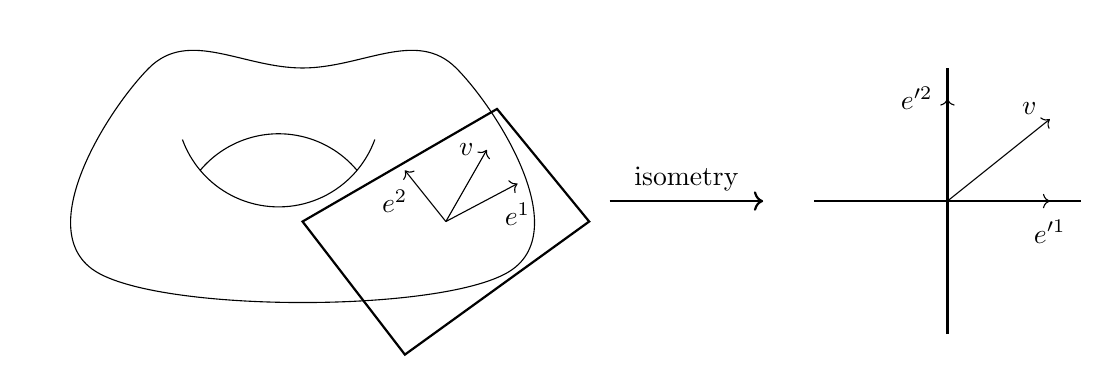
\begin{tikzpicture}[scale=1.3]
		\draw[smooth cycle,tension=.7] plot coordinates{(0,0) (0.5,2) (2,2) (3.5,2) (4,0)};
		\coordinate (A) at (1,1);
		\draw (A) arc(140:40:1) (A) arc(-140:-20:1) (A) arc(-140:-160:1);
		
		
		\draw[thick] (2,0.5) -- (3,-0.8) -- (4.8,0.5) -- (3.9,1.6) -- cycle;
		% 标注e1和e2
		\draw[->] (3.4,0.5) -- (4.1,0.87);
		\draw[->] (3.4,0.5) -- (3.0,1);
		\node at (4.1,0.57) {\(e^1\)};
		\node at (2.9,0.7) {\(e^2\)};
		
		% 标注v向量
		\draw[->] (3.4,0.5) -- (3.8,1.2);
		\node at (3.6,1.2) {\(v\)};
		
		% 等距映射箭头
		\draw[->, thick] (5,0.7) -- (6.5,0.7) node[midway, above] {isometry};
		
		% 绘制右侧的欧几里得平面
		\draw[thick] (7,0.7) -- (9.6,0.7);
		\draw[thick] (8.3,-0.6) -- (8.3,2);
		
		% 标注e1'和e2'
		\draw[->] (8.3,0.7) -- (9.3,0.7);
		\draw[->] (8.3,0.7) -- (8.3,1.7);
		\node at (9.3,0.4) {\(e'^1\)};
		\node at (8.0,1.7) {\(e'^2\)};
		
		% 标注v'向量
		\draw[->] (8.3,0.7) -- (9.3,1.5);
		\node at (9.1,1.6) {\(v\)};
		
	\end{tikzpicture}
	\caption{Isometry}
\end{figure}
%



\subsubsection{Upper Bound of \texorpdfstring{$\lambda_m$}{lambda\_m}}
\label{sec:phim-lambdam}


The most classical result for estimating eigenvalues is Weyl's law:
\begin{align}
N(\lambda)\sim \frac{\omega(d) Vol(M) \lambda^\frac{d}{2}}{(2\pi)^{d}},
\end{align}
where $N(\lambda)$ is the number of eigenvalues less than or equal to $\lambda$. 

If we ask $\lambda=\lambda_k$, the above is equivalent to
\begin{align}
	\lambda_k^{d/2} \sim \frac{(2\pi)^d k}{\omega(n) Vol(M)}
\end{align}

Weyl's law provides an asymptotic expression for the eigenvalues of the Laplace--Beltrami operator, offering profound insights into their growth rates. However, in our paper, strict control for eigenvalues is essential. This requires not only asymptotic estimates but also rigorous upper bounds that hold universally. A notable result for the upper bound was established by Li--Yau \cite[Thm. 16]{esteigenvalue}, who derived explicit upper bounds for the eigenvalues under geometric constraints, which align with the assumptions in our study.


We estimate the upper bound of eigenvalues. If the lower bound of the Ricci curvature $\kappa_M$ of $M$ is less than $0$, we have 
\begin{align}
	\lambda_k \leq 
	\left\{
	\begin{array}{l}
		\displaystyle \frac{(2\beta+1)^2}{4}(-\kappa_M) + 4(1+2^\beta)^2\pi^2 \left(\frac{\sinh \sqrt{-\kappa_M}\text{diam}}{\sqrt{-\kappa_M}\text{diam}}\right)^\frac{2d-2}{d} \\
		\hspace{10em} \times \left((k+1)\frac{\alpha(d-1)}{d}\frac{1}{V}\right)^\frac{2}{d} \\[1.5ex]
		\text{when } d=2(\beta+1), \beta = 0,1,2\dots \\[2.5ex]
		\displaystyle \frac{(2\beta+2)^2}{4}(-\kappa_M) + 4(1+\pi^2)(1+2^{2\beta})^2 \left(\frac{\sinh \sqrt{-\kappa_M}\text{diam}}{\sqrt{-\kappa_M}\text{diam}}\right)^\frac{2d-2}{d} \\
		\hspace{10em} \times \left((k+1)\frac{\alpha(d-1)}{d}\frac{1}{V}\right)^\frac{2}{d} \\[1.5ex]
		\text{when } d=2\beta+3, \beta = 0,1,2\dots
	\end{array} 
	\right. ,
\end{align}


if $M$ has non--negative Ricci curvature $\kappa_M$, we have
\begin{align}
	\lambda_k \leq (d+4)d^{1-\frac{2}{d}}\left(\frac{k+1}{V}\alpha(d-1)\right)^\frac{2}{d} ,
\end{align}
where $d$ is the dimension of $M$, $V$ is the volume of $M$ and $\alpha(n)$ is the volume of $S^n$ in $\mathbb{R}^{n+1}$.\cite{esteigenvalue}

Since for $M \in \mathcal{M}$, the volume is greater that $V_1$ and the lower bound of the Ricci curvature is greater than $\kappa$, so $\frac{1}{V}\leq \frac{1}{V_1}$ and $-\kappa_M\leq -\kappa$, thus we have 
\begin{align}
	\lambda_k \leq \left\{
	\begin{array}{cc}
		C(d,V) (k+1)^\frac{2}{d} \quad &\text{if } \kappa_M \text{ is non-negative} \\
		C(d,\kappa,\text{diam},V) (k+1)^\frac{2}{d} \quad  &\text{if } \kappa_M \text{ is negative}
	\end{array}
	\right. .
\end{align}
Summarizing above, we have
	\begin{lemma}[Uniform upper bound on $\lambda_k$]
	\label[lemma]{lem:lambdam-bound}
	There exists a constant $C(\MM)$, depending only on the uniform geometric parameters $(d,\kappa,\mathrm{diam},V)$ of the family $\MM$, such that
	\begin{align}
		\lambda_k \leq C(\MM) (k+1)^\frac{2}{d} \qquad \text{for all } M \in \MM.
	\end{align}
\end{lemma}



\subsubsection{Estimate of Higher Order Derivatives}
\label{sec:phim-higher-deri}

In this subsection, we will estimate the $L^\infty$ norm of higher order derivatives for eigenfunctions to control the operator norm of $d N^\prime$ in the next subsection.  

One similar result is Bernstein inequality, for eigenfunction $e_\lambda$ of $\Delta$: $\Delta e_\lambda =\lambda e_\lambda$, we have\cite{xu2009gradient}:
\begin{align}
	\|\nabla e_\lambda\|_{L^\infty}\leq C\lambda^{\frac{1}{2}} \|e_\lambda\|_{L^\infty}
\end{align}


\cite{xu2005asymptotic} proved a more general estiamte, for eigenfunction $e_\lambda$ of $\Delta$: $\Delta e_\lambda =\lambda e_\lambda$, we have 
\begin{align}
	\|e_\lambda\|_{H^\infty_k}\sim \lambda^\frac{k}{2} \|e_\lambda\|_{L_\infty} \quad \text{as }\lambda \rightarrow \infty
\end{align}
where $\sim$ means the equivalence between two norms, and $\|\cdot\|_{H^k_\infty}$ is Sobolev norm. If we revise this result to have a upper bound (the author says we only need a little effort to do so), we can control $\|d^k \varphi\|$ since we have had the upper bound of $\lambda_m$ which only depend on $M$.

\cite{2004Xuhigherorder} also gave a better estimate:
\begin{align}
	\|e_\lambda(x)\|_{H^\infty_k} \leq C \lambda^{k/2+(d-1)/4}\|e_\lambda(x)\|_{L^2}
\end{align}
however, $C$ may not be an uniform constant for $M \in \mathcal{M}$.


To estimate the $L^\infty$ norm of derivatives for eigenfunctions, we first choose the coordinate chart to be normal coordinate chart to make our derivatives well defined. We take derivative of $e(x): M \rightarrow \R$ in the following sense: Let $x \in U$ be the normal coordinate chart $(U,\textbf{x})$ and $\hat{U}=\textbf{x}(U)$, then $\hat{e}(x)=e\circ \textbf{x}^{-1}:\hat{U}\rightarrow R$ be the coordinate representation of $e(x)$. We treat $\partial_i e(x)$ as $\partial_i \hat{e}(x)$, and for higher order derivatives as well.

\begin{lemma}[Uniform bound on the higher derivatives of the eigenfunctions]
	\label[lemma]{lem:eigfn-deri-bound}
	For every multi--index $\alpha$ with $|\alpha| \leq k$ there exists a constant $C_\alpha$, depending only on $\alpha$ and the uniform geometric parameters of $\MM$, such that the eigenfunction derivatives satisfy the pointwise bound
	\begin{align}
		|\partial^\alpha e_\lambda(x)| \leq C_\alpha (1+\lambda)^{k/2+d/4}, \qquad |\alpha| \leq k.
	\end{align}
\end{lemma}
 Consequently, since $\lambda_k$ is bounded above by $C(\MM)(k+1)^\frac{2}{d}$, $\varphi_j = (2t)^\frac{d+2}{4}\sqrt{2}(4\pi)^\frac{d}{4}e^{-\lambda_1 t}e_j(x)$, then the coordinate derivatives of $\varphi$ up to order $k$ are uniformly bounded over $M \in \MM$.

\begin{proof}[Proof of \cref{lem:eigfn-deri-bound}]
Let $\gamma$ be a $2d$ multi--index with $|\gamma|:=\sum_i\gamma_i\leq k$, and $x,y \in U$ be a geodesic normal coordinate of $M$. We denote $\sum_{\lambda_j\leq \lambda} e_j(x) e_j(y)$ as $e(x,y,\lambda)$. Let $\gamma = \left(\gamma_1,\dots,\gamma_{2d}\right)$, then the $\gamma$ order derivative for $e_j(x) e_j(y)$ is 
\begin{align}
	\partial^\gamma_{x,y} e_j(x) e_j(y) = \frac{\partial^{|\gamma_1+\cdots+\gamma_{d}|}e_j(x)}{\partial x_1^{\gamma_1} \cdots \partial x_d^{\gamma_d}} \frac{\partial^{|\gamma_{d+1}+\cdots+\gamma_{2d}|}e_j(y)}{\partial y_1^{\gamma_{d+1}} \cdots \partial y_d^{\gamma_{2d}}}
\end{align}

We have \cite[Lem. 2.4]{2004Xuhigherorder}
\begin{align}
	|\partial^\gamma_{x,y}e(x,y,\lambda)|\leq C_\gamma (1+\lambda)^{\frac{d+|\gamma|}{2}}.
\end{align}

To have the estimate for derivatives of eigenfunctions, let $\alpha$ be a $d$ dimension multi--index, and using the inequality above with $\gamma = \left(\alpha , \alpha\right)$, then we have 
\begin{align}
	|\partial^\alpha e_\lambda (x)|^2\leq\sum\limits_{\lambda_j\leq \lambda} |\partial^\alpha e_j(x)|^2 \leq C_\alpha (1+\lambda)^{d/2+|\alpha|}
\end{align}
so
\begin{align}
	\label{deriinequ}
	\|e_\lambda\|_{H^\infty_k}=\max\limits_{|\alpha|\leq k}|\partial^\alpha e_\lambda(x)|\leq \sup\limits_{|\alpha|\leq k}\left\{C_\alpha\right\}(1+\lambda)^{k/2+d/4}
\end{align}
Since $\lambda_k$ is bounded above by $C(\MM) (k+1)^{\frac{2}{d}}$, which implies that $\|\varphi_j\|_{H_k^\infty}\leq C(l)$ for $\varphi_j:M \rightarrow \mathbb{R}$. Therefore, $|\frac{\partial^l \varphi_j}{\partial x_{i_1}\cdots\partial x_{i_l}}| \leq C(l)$ for $l\leq k$ with respect to normal coordinate.
\end{proof}

After deriving the uniform bound for the norm of the derivatives of $\phi$, we now establish the bound of the operator norm of the covariant derivatives.
\begin{lemma}[Uniform bound on the higher derivatives of the embedding map $\varphi$]
	\label[lemma]{lem:covar-deri-bound}
	For every $l \leq k$ there exists a constant $A(l)$, depending only on $l$ and the uniform geometric parameters of $\MM$, such that the operator norm of the $l$-th derivative of the embedding map is bounded uniformly over $\MM$:
	\begin{align}
		\|d^l \varphi\| \leq \sqrt{m}\,A(l)\,d^{l/2} \quad \text{for all }M \in \MM.
	\end{align}
\end{lemma}

\begin{proof}[Proof of \cref{lem:covar-deri-bound}]
By \cref{lem:eigfn-deri-bound}, the coordinate derivatives of $\varphi$ up to order $k$ are uniformly bounded over $M \in \MM$; we use this together with the uniform bounds on the Christoffel symbols and their derivatives to control $\|d^l\varphi\|$.

To estimate the norm of $d\varphi$, we can derive its local coordinate representation and compute the covariant derivatives in the normal chart since  choosing different chart does not have the influence on the norm. Now we denote $\varphi$ as $j$--th component of $\varphi$ to simplify the notation and let $(U,\textbf{x})$ be the normal chart.

For the first order covariant derivative, we have
\begin{align}
	\nabla \varphi (X) = \nabla_X \varphi = X\varphi,
\end{align} 
thus 
\begin{align}
	\nabla \varphi = \varphi_i dx^i\quad  \text{with}\ \varphi_i = \partial_i \varphi,
\end{align}
so for the first order covariant derivative, the local coordinate representation is the first order derivative of local representation of $\varphi$.

For second order covariant derivative, which is also known as covariant Hessian. We have 
\begin{align}
\nabla^2 \varphi (X,Y)= \nabla^2_{Y,X}=\nabla_Y(\nabla_X \varphi)-\nabla_{\nabla_Y X}\varphi=X(Y\varphi)-(\nabla_X Y)\varphi
\end{align}
thus in local coordinates,
\begin{align}
	\nabla^2 \varphi = \varphi_{ij} dx^i \otimes dx^j \quad \text{with}\ \varphi_{ij}=\partial^2_{ij}\varphi-\Gamma^k_{ij}\partial_k \varphi,
\end{align}
%
with $i,j,k\in\{1,2,\ldots d\}$. 
For the third order coordinate derivative, we have 
\begin{align}
	\nabla^3 \varphi (X,Y,Z)&=(\nabla_Z \nabla^2 \varphi) (X,Y)\\
	&=Z(\nabla^2 \varphi (X,Y))-\nabla^2\varphi (\nabla_Z X,Y)-\nabla^2 \varphi (X,\nabla_Z Y)\\
	&=Z(X(Y\varphi)-(\nabla_X Y)\varphi)-\nabla_Z X(Y\varphi)+(\nabla_{\nabla_Z X} Y)\varphi \nonumber \\
	&\qquad\qquad \quad -X(\nabla_Z Y\varphi)+(\nabla_X \nabla_Z Y)\varphi,
\end{align}
thus in the local coordinate, 
\begin{align}
 \nabla^3 \varphi =\varphi_{ijk} dx^i \otimes dx^j \otimes dx^k &\\
 \text{with}\quad \varphi_{ijk}=\partial^3_{ijk} \varphi- \partial_k \Gamma_{ij}^l \partial_l \varphi - \Gamma_{ij}^l \partial^2_{kl}\varphi-\Gamma_{ik}^m\partial^2_{mj} \varphi&+ \Gamma_{ik}^l \Gamma_{lj}^m \partial_m \varphi-\partial_i \Gamma_{jk}^l \partial_l \varphi \nonumber\\
 & -\Gamma_{jk}^l \partial^2_{il}\varphi+ \Gamma_{il}^m\Gamma_{jk}^l\partial_m \varphi.
\end{align}

The local coordinate representation is combined with derivative of Christoffel symbol and third order derivative of $\varphi$. And we can prove easily by induction that the local coordinate representation of $\nabla^l \varphi$ is $\varphi_{i_1\cdots i_l} dx^{i_1} \otimes \cdots \otimes dx^{i_l}$
with $\varphi_{i_1\cdots i_l}$ can be represented by derivative of $\varphi$ not higher than order $l$ and derivative of Christoffel symbol not higher than order $l-2$. To prove this, we only need to notice that 
\begin{align}
	\nabla^{l+1}\varphi(X_1,\cdots,X_l,X)&=\nabla(\nabla^l \varphi)(X_1,\cdots,X_l,X) \\
	&=(\nabla_X \nabla^l \varphi) (X_1,\cdots,X_l)\\
	&=X(\nabla^l \varphi(X_1,\cdots,X_l))-\sum_{i=1}^l \nabla^l\varphi(X_1,\cdots,\nabla_X X_i,\cdots,X_l)
\end{align}

Since we assume for any $M \in \mathcal{M}$, the local coordinate
representation in the normal chart of the Christoffel symbols and
their derivatives with order not above $k-2$ have an uniform bound only depends on its order,
and we have claimed derivatives of $\varphi$ which order is not higher
than $k$ have an uniform bound, and we notice that the local
representation of $\nabla^k \varphi$ is combined with them in the same
pattern among all $M \in \mathcal{M}$. Therefore, $\varphi_{i_1\cdots
  i_l}$ is bounded uniformly for all $l \leq k$, i.e.
\begin{align}
|\varphi_{i_1\cdots i_l}| \leq A(l) \quad \text{for }l\leq k
\end{align}


With this control of upper bound, we can estimate the norm of higher derivatives of $\varphi$:
\begin{align}
	\|d^l \varphi\|&=\sup\limits_{\|v_1\|=1, \dots,\|v_l\|=1} \|\nabla^l \varphi (v_1,\dots,v_l)\| \\
	&=\sup\limits_{\|v_1\|=1, \dots,\|v_l\|=1} \|\nabla^l \varphi (v_1\otimes\dots\otimes v_l)\| \\
	&=|\varphi_{i_1\cdots i_l} dx^{i_1} \otimes \cdots \otimes dx^{i_l} (v_1^{i_1} \frac{\partial}{\partial x^{i_1}} \otimes \cdots \otimes v_l^{i_l} \frac{\partial}{\partial x^{i_l}})|\\
	&=|\varphi_{i_1\cdots i_l} v_1^{i_1} \cdots v_l^{i_l}| \\
	&\leq A(l) \left|\sum_{i_1,i_2,\dots i_l=1}^d   v_1^{i_1} \cdots v_l^{i_l}\right|\\
	&= A(l) \left|\sum_{i_1=1}^{d} v_1^{i_1} \sum_{i_2,\dots i_l=1}^dv_2^{i_2} \cdots v_l^{i_l}\right|\\
	\text{(AM-–GM)}&\leq A(l) \left|\sum_{i_2,\dots i_l=1}^dv_2^{i_2} \cdots v_l^{i_l}\right| \sqrt{d}\\
	&\ \ \vdots \\
	&\leq A(l) d^{l/2}.
\end{align}

This inequality holds for all $l \leq k$. Here $\varphi : M \rightarrow \mathbb{R}$, thus $d^l \varphi (v_1,\dots,v_l)$ gives a vector in $\mathbb{R}$, and then $d^l \varphi (v_1,\dots,v_l) = \left(d^l\varphi_1(v_1,\dots,v_l),\dots,d^l\varphi_m (v_1,\dots,v_l)\right)$ is a vector in $\mathbb{R}^m$, which is also a tangent vector in $T_{\varphi(p)}\varphi(M)$ through the natural isometry. Since $d^l \varphi(v_1,\dots,v_l)$ has $m$ components, it is easy to check the operator norm of $d^l \varphi$ has the upper bound $\sqrt{m}A(l)d^{l/2}$. Therefore, $\|d^l \varphi\|$ are bounded uniformly for $l \leq k$.
\end{proof}
\subsection{Uniform upper bounds  \texorpdfstring{$\left\{L_{\perp},L_3,\dots,L_k\right\}$}{L\_perp,L\_3, \dots, L\_k} on the higher derivatives of the local parametrization reminder}
\label{sec:phim-L}

In this section, we will verify that there exists an common parameter set $\textbf{L}^\prime:=\left\{L_{\perp}^\prime,L_3^\prime,\dots,L_k^\prime\right\}$ such that the operator norm of the derivatives of remainder $N_{\varphi(p)}$ defined in Assumption \ref{as:smooth} can be controlled uniformly over $\varphi(\MM)$, which is builded on the uniform bound on $\|d^l \varphi\|$ from \cref{lem:covar-deri-bound}.

\begin{lemma}[Uniform control of the parametrization remainder]
	\label{lem:remainder-bound}
	There exists a common parameter vector $\textbf{L}^\prime:=\left(L_\perp^\prime,\dots,L_k^\prime\right)$, depending only on the uniform geometric parameters of $\MM$, such that for every $M \in \MM$ and every $p^\prime=\varphi(p) \in \varphi(M)$ the local parametrization remainder $N^\prime_{p^\prime}$ satisfies $N^\prime_{p^\prime}(0)=0$, $d_0 N^\prime_{p^\prime}=0$, and
	\begin{align}
		\|d^l_{v^\prime} N^\prime_{p^\prime}\| \leq L_l^\prime \qquad \text{for } 2 \leq l \leq k.
	\end{align}
\end{lemma}

\begin{proof}[Proof of \cref{lem:remainder-bound}]
We fix a point $p^\prime=\varphi(p) \in \varphi(M)$, for $v^\prime \in T_{p^\prime}\varphi(M)=d\varphi_p(T_pM)$, we define 
\begin{align}
	\Psi^\prime_{p^\prime}(v^\prime)=\varphi(\Psi_p(d(\varphi^{-1})_{p^\prime} (v^\prime)))=p^\prime+v^\prime+N^\prime_{p^\prime}(v^\prime)
\end{align}
from definition of $\Psi_p$, we know $\Psi^\prime_{p^\prime}(v^\prime)$ and $N^\prime_{p^\prime}(v^\prime)$ are well defined when $\Vert d(\varphi^{-1})_{p^\prime}(v^\prime)\Vert \leq \frac{1}{4L_\perp}$. 

We estimate $\|d \varphi^{-1}_{p^\prime}\|$: We can treat $T_p M$ as a
$d$ dimensional subspace of $\mathbb{R}^D$ and treat $T_{p^\prime}
\varphi(M)$ is a  $d$ dimensional subspace of $\mathbb{R}^m$, and these
inclusions are canonical and isometric, so they are both closed
subspaces. And $d \varphi_p$ is homeomorphism, so graph of $d
\varphi^{-1}_{p^\prime}$ is closed, then $d \varphi^{-1}_{p^\prime}$
is bounded, i.e. $\|d \varphi^{-1}_{p^\prime}\|$ exists.
\begin{align}
	\|d \varphi^{-1}_{p^\prime}\|&=\sup \left\{\|d\varphi^{-1}_{p^\prime} v^\prime \|: v^\prime \in Im(d\varphi_p), \|v^\prime\| = 1\right\} \\
	&=\sup \left\{\frac{\|v\|}{\|d\varphi_p v\|}: v^\prime \in Im(d\varphi_p), \|v^\prime\| = 1, v=d \varphi^{-1}_{p^\prime} v^\prime\right\} \\
	&=\sup \left\{\frac{1}{\|d\varphi_p v\|}: \|v\| = 1\right\} \\
	&\leq \frac{1}{1-\epsilon}
\end{align}
so when $\|v^\prime\| \leq \frac{1}{4L_\perp(1-\epsilon)}$, $\Vert d(\varphi^{-1})_{p^\prime}(v^\prime)\Vert \leq \frac{1}{4L_\perp}$, then $\Psi^\prime_{p^\prime}(v^\prime)$ and $N^\prime_{p^\prime}(v^\prime)$ are well defined.


Now, We check $N^\prime_{p^\prime}(0)=0$ and $d_0N^\prime_{p^\prime}=0$:
\begin{align}
	N^\prime_{p^\prime}(0)+p^\prime=\varphi(\Psi_p(d(\varphi^{-1})_{p^\prime}(0)))=\varphi(\Psi_p(0))=\varphi(p+0+N_p(0))=\varphi(p)=p^\prime\\
	d_0N^\prime_{p^\prime}=d\varphi_p d_0\Psi_p d(\varphi)_{p^\prime}^{-1}-I_m=d\varphi_p(I_D+d_0N_p) d(\varphi)_{p^\prime}^{-1}-I_m=0
\end{align}

We assume $\|v^\prime\| \leq \frac{1}{4L_\perp(1-\epsilon)}$ and denote $d\varphi_{p^\prime}^{-1}v^\prime$ as $v$, and $c(v^\prime)=p+v+N_p(v)$, then for any unit vector $w^\prime \in T_{p^\prime} \varphi(\mathcal{M})$, using Faà di Bruno's formula, we have
\begin{align}
	\left\|d^k_{v^\prime}N^\prime_{p^\prime}(w^{\prime \otimes k})\right\| \!= \! \left\| \sum\limits_{\pi \in P(k)} \! d^l_{c(v^\prime)} \varphi \circ \! \left(d^{j_1}_v \Psi_p \! \left(\left\{d_{p^\prime}\varphi^{-1} w^\prime\right\}^{\otimes j_{1}}\right),\dots,d^{j_l}_v \Psi_p \! \left(\left\{d_{p^\prime}\varphi^{-1} w^\prime\right\}^{\otimes j_{l}}\right) \right)\right\|,
\end{align}
where $P(k)$ is a partition of $k$ with $l$ parts such that $j_1+\dots+j_l=k$.


Since $\Psi_p(v)=p+v+N_p(v)$, so $d_v \Psi_p = I+ d_v N_p$, $d^i_v \Psi_p = d^i_v N_p$, thus
\begin{align}
	\|d_v \Psi_p\| = \| I+ d_v N_p \| \leq 1 + L_\perp \|v\| \\
	\|d^i_v \Psi_p\| =\|d^i_v N_p\| \leq L_i
\end{align}
therefore
\begin{align}
\|d^k_{v^\prime}N^\prime_{p^\prime}(w^{\prime \otimes k})\| &\leq \sum\limits_{\pi \in P(k)} \|d^l \varphi\| \prod_{i=1}^l \| d^{j_i} \Psi_p\| \|d_{p^\prime}\varphi^{-1} w^\prime\|^{j_i} \\
&\leq \sum\limits_{\pi \in P(k)} \|d^l \varphi\| \frac{1}{(1-\epsilon)^l} \prod_{i=1}^l \| d^{j_i} \Psi_p\| 
\end{align}


We have proved $\|d^j \varphi\|$ and $\|d^j_v \Psi_p\|$ have the uniform upper bound for $j=2,\dots,k$ in \cref{lem:covar-deri-bound}, so we can select $\textbf{L}^\prime:=\left(L_\perp^\prime,\dots,L_k^\prime\right)$ as the uniform upper bound of $\|d^2_{v^\prime}N^\prime_{p^\prime}\|,\dots,\|d^k_{v^\prime}N^\prime_{p^\prime}\|$.
\end{proof}

\subsection{Bounds on the pushforward density}
\label{sec:density}

In this subsection, we estimate the pushforward density of the sampling process. By establishing both lower and upper bounds for the pushforward density, we ensure that the sampling over $\varphi(M)$ remains approximately uniform. This guarantees that there are always some sampling points in any nonzero measure region with nonzero probability, thereby allowing the manifold to be effectively approximated using the sampled points.

\begin{lemma}[Almost-uniform pushforward density]
	\label{lem:density-bound}
	Suppose $\epsilon \leq \frac{1-4^{-1/d}}{3}$. Then for every $M \in \MM$ the Jacobian factor of $\varphi$ satisfies
	\begin{align}
		\sqrt{\det \left(\pi_{T_p M} \circ d\varphi_p^T \circ d\varphi_p |_{T_pM}\right)} \in \left(\tfrac{1}{2},2\right),
	\end{align}
	and consequently the pushforward density $g$ of $\varphi_\# P$ obeys $\tfrac{f_{\min}}{2} < g < 2 f_{\max}$. 
\end{lemma}

\begin{proof}[Proof of \cref{lem:density-bound}]
We denote $d\varphi_p:T_p M \rightarrow T_{p^\prime} N$ as $A$, then for $\|v\|=1$, $1-\epsilon<\|Av\|<1+\epsilon$, which means $\|A\|<1+\epsilon$, so $\sqrt{\lambda_{\max}(A^T A)}<1+\epsilon$. We know $A^T A$ is positive-definite  symmetric matrix, we consider an unit eigenvector $v$ of it with eigenvalue $\lambda$, then 
\begin{align}
	\lambda=\|v^T \lambda v\|= \|v^T A^T A v\|=\|Av\|^2\in ((1-\epsilon)^2,(1+\epsilon)^2).
\end{align}

Since $A^TA$ is symmetric, then $A^T A=Q\Lambda Q^T$,  where $Q$ is orthogonal matrix and $\Lambda$ is diagonal matrix whose diagonal elements are eigenvalues of $A^T A$ and all of them are close to $1$.
\begin{align}
	|\|\pi_{T_p M} A^T A v\|-\|v\||&\leq \|\pi_{T_p M}(A^T A -I) v\|\\
	&=\|\pi_{T_p M} Q(\Lambda-I)Q^T v\|\\
	&\leq \|Q(\Lambda-I)Q^T v\|\\
	&\leq 3\epsilon,
\end{align}
the last inequality is due to orthogonal matrix does not change norm of vector and diagonal elements in $\Lambda-I$ are smaller than $3\epsilon$.

Thus we have $1-3\epsilon <\|\pi_{T_p M} A^T A v\|<1+3\epsilon $, so the eigenvalues of $\pi_{T_p M} A^T A|_T$ is greater than $1-3\epsilon$ and less than $1+3\epsilon$. Therefore, if 
\begin{align}
	\label{range_of_e}
	\epsilon \leq \min\left\{\frac{4^{1/d}-1}{3},\frac{1-\frac{1}{4^{1/d}}}{3}\right\} = \frac{1-\frac{1}{4^{1/d}}}{3},
\end{align}
then
\begin{align}
	\det (\pi_{T_p M} A^T A|_T)=\prod \lambda_i\in ((1-3\epsilon)^d,(1+3\epsilon)^d)\subset(\frac{1}{4},4),
\end{align}
which implies
\begin{align}
	\sqrt{\det \left(\pi_{T_p M} \circ d\varphi_p^T \circ d\varphi_p |_{T_pM}\right)} \in (\frac{1}{2},2).
\end{align}

According to \cref{thm:push_density}, we have the pushforward density of $\varphi_\# P$ is 
	\begin{align}
	g(p^\prime)=f(p)/\sqrt{\det \left(\pi_{T_p M} \circ d\varphi_p^T \circ d\varphi_p |_{T_pM}\right)},
\end{align}
where $p^\prime = \varphi(p)$. Therefore, $\frac{f_{min}}{2}<g<2f_{\max}$.
\end{proof}

In our setting, our sampleing is uniform, thus $f \equiv \frac{1}{Vol(M)}$, which is bounded from both and above, which implies the density of $\varphi(\MM)$ is also bounded from below by $\min\limits_{M \in \MM} \left\{Vol(M)\right\}/2$ and bounded above by $2\max\limits_{M \in \MM} \left\{Vol(M)\right\}$.

\subsection{Estimation of \texorpdfstring{$\tau_{\min}$}{tau-min}}
\label{sec:reach}

    If $M$ has reach $\tau$, then at least one
  of the following cases holds:
\begin{enumerate}
	\item[I] (Global case) $M$ has a bottleneck, i.e. there exist $p, q \in M$, such that $(p+q)/2 \in \text{Med}(M)$ and $\|p-q\|=2\tau$.
	\item[II] (Local case) There exists $p \in M$, and an arc-length parametrized geodesic $\gamma$ such that $\gamma(0)=p$ and $|\gamma^{\prime\prime}(0)|=1/\tau$.
\end{enumerate}
where $\text{Med}(M)=\left\{z\in \mathbb{R}^D: \exists p\neq q\in M, \|z-p\|=\|z-q\|=d_E(z,M) \right\}$, $d_E(x,M)$ is the distance between $x$ and $M$.

We denote global reach and local reach as $\tau_g$ and $\tau_l$, respectively. Thus $\tau = \min \left\{\tau_g, \tau_l\right\}$

\begin{figure}[H]
	\centering
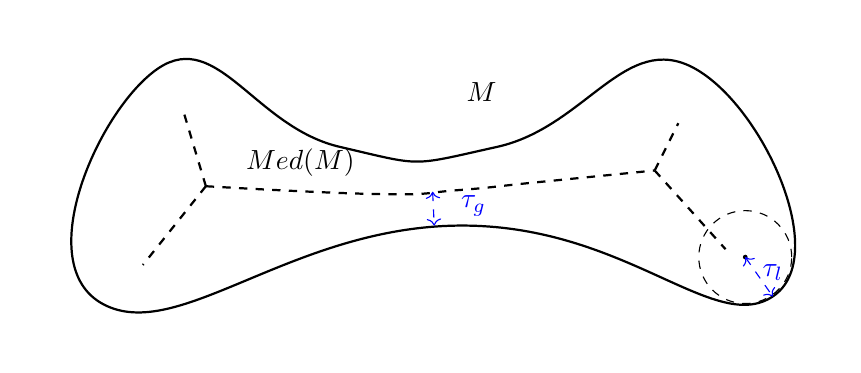
\begin{tikzpicture}
	
	% 绘制M的不规则形状
	\draw[thick] plot [smooth cycle, tension=0.9] coordinates {(-4.5,-1.5) (-3.8,1.5) (-1.5,0.5) (0.5,0.5) (3,1.5) (4,-1.4) (0,-0.5) };
	\draw[dashed] (3.65,-0.9) circle [radius=0.59];
	\fill (3.65,-0.9) circle [radius=0.03];
	\draw[<->, dashed, blue] (3.65,-0.9) -- (4,-1.4);
	
	\node[blue]  at (4.0,-1.1) {\(\tau_l\)};
	% 绘制中轴线Med(M)
	\draw[dashed, thick] plot [smooth, tension=0.8] coordinates {(-3.2,0) (-1,-0.1) (0,-0.05) (1,0.05) (2.5,0.2)};
	
	% 绘制两端的分叉
	\draw[dashed, thick] (-3.2,0) -- (-4,-1);
	\draw[dashed, thick] (-3.2,0) -- (-3.5,1);
	\draw[dashed, thick] (2.5,0.2) -- (3.4,-0.8);
	\draw[dashed, thick] (2.5,0.2) -- (2.8,0.8);
	
	% 绘制TM距离的箭头
	\draw[<->, dashed, blue] (-0.32,-0.07) -- (-0.3,-0.5);
	
	% 标注文字
	\node[blue] at (0.2,-0.25) {\(\tau_g\)};
	\node at (0.3,1.2) {\(M\)};
	\node at (-2,0.3) {\(Med(M)\)};
	
\end{tikzpicture}
	\caption{Reach}
\end{figure}

We can define $\tau_l$ easily by 
\begin{align}
	\tau_l := \inf\limits_{p\in M} \left\{\frac{1}{\|\mathrm{II}_p\|}\right\}.
\end{align}

We will show that there exists a uniform positive lower bound on the reach of $\varphi(M)$ for all $\varphi(M) \in \varphi(\MM)$:
\begin{theorem}[Uniform lower bound on the reach of $\varphi(\MM)$]
	\label{thm:reach-bound}
	There exists a positive constant $\tau_{\varphi(\MM)}$, depending only on the uniform geometric parameters of $\MM$ and on the DM parameters $(m,t_0)$, such that
	\begin{align}
		\tau_{\varphi(M)} \geq \tau_{\varphi(\MM)} > 0 \qquad \text{for all } M \in \MM.
	\end{align}
\end{theorem}
The bound is obtained by writing $\tau = \min\{\tau_l,\tau_g\}$ and bounding each term separately: the local reach is controlled through the second fundamental form of $\varphi(M)$ (\cref{lem:local-reach}), and the global reach is controlled in \cref{sec:glo-reach}.







%%% Using geodesic curvature

\iffalse
%now we prove in normal coordinate chart of $M$, $|\frac{\partial f_i}{\partial x_k}|$ and $|\frac{\partial^2 f_i}{\partial x_k \partial x_p}|$ are bounded. We consider a curve $(tv^1,tv^2,...,tv^d) \subset \hat{U}$, then $(f_1(tv^1,tv^2,...,tv^d),...,f_D(tv^1,tv^2,...,tv^d))$ is the geodesic starting at $p$ with initial velocity $v^i\partial_i(p) \in T_pM$. We take $v^k=1$ and others equal $0$, then $(\frac{\partial f_1}{\partial x_k},...,\frac{\partial f_D}{\partial x_k})(0,...,t,...,0)$ is the unit tangent vector along this geodesic， thus $|\frac{\partial f_i}{\partial x_k}|\leq 1$. We take second order derivative, and use the assumption $|\gamma^{\prime \prime}(s)|$ is bounded, we obtain $|\frac{\partial^2 f_i}{\partial x_k^2}|$ is also bounded. If we ask $v^k= v^p = \frac{\sqrt{2}}{2}$ and take second order derivative, we have $|\frac{\partial^2 f_i}{\partial x_k^2}+2\frac{\partial^2 f_i}{\partial x_k\partial x_p}+\frac{\partial^2 f_i}{\partial x_p^2}|$ is bounded, since $|\frac{\partial^2 f_i}{\partial x_k^2}|$ is bounded, by triangle inequality, $|\frac{\partial^2 f_i}{\partial x_k \partial x_p}|$ is bounded


Using tangent vector, we obtain the metric tensor, whose $(i,j)$ component is 
\begin{align}
	g_{ij}=\left\langle r_i,r_j\right\rangle 
\end{align}
we take partial derivative of it, we have 
\begin{align}
	\frac{\partial g_{ij}}{\partial x_k}=\left\langle r_i , \frac{\partial r_j}{\partial x_k}\right\rangle + \left\langle \frac{\partial r_i}{\partial x_k} , r_j\right\rangle 
\end{align}
we have proved $|\frac{\partial^2  \varphi_i}{\partial x_k \partial x_p}|$ and $|\frac{\partial \varphi_i}{\partial x_k}|$ are bounded, so $\frac{\partial g_{ij}}{\partial x_k}$ is bounded since both $r_i$ and $\frac{\partial r_j}{\partial x_k}$ are bounded.

The Christoffel symbol is 
\begin{align}
	\Gamma^\lambda_{\mu\nu} = \frac{1}{2} g^{\lambda\sigma} \left( \frac{\partial g_{\sigma\nu}}{\partial x^\mu} + \frac{\partial g_{\sigma\mu}}{\partial x^\nu} - \frac{\partial g_{\mu\nu}}{\partial x^\sigma} \right)
\end{align}
where $g^{\lambda \sigma}$ is the inverse matrix of $g_{ij}$, so $g^{\lambda \sigma}=\frac{1}{det(g)} det(C_{\lambda \sigma})$ is also bounded, where $C_{\lambda \sigma}$ is the $(\lambda, \sigma)$ cofactor. Now we consider the lower bound of $det(g)$, we have
\begin{align}
	g_{ij}=\left\langle r_i,r_j\right\rangle = \sum_{k=1}^m \frac{\partial \hat{\varphi}_k}{\partial x_i} \frac{\partial \hat{\varphi}_k}{\partial x_j}
\end{align}
thus $g=J^T J$, where $J=\left(\frac{\partial \hat{\varphi}_i}{\partial x_j}\right)\ i=1,\dots,m, \ j=1,\dots,d
$. We have proved the eigenvalues of $J^TJ$ is close to $1$, so $det(g)= det(J^TJ)$ is bounded below. Therefore, Christoffel symbols are bounded uniformly.




We consider a geodesic $\gamma(t)$ passing through $\varphi(p) \in V \subset \varphi(M)$, its coordinate representation is $(z_1(t),\dots,z_d(t))$. According to geodesic equation, we have 
\begin{align}
	\frac{d^2 z_k}{dt^2}+\Gamma_{ij}^k\frac{dz_i}{dt}\frac{dz_j}{dt}=0, \quad k=1,2,\dots,d
\end{align}

$\dot{z}(0)=(\frac{dz_1}{dt}(0),\dots,\frac{dz_d}{dt}(0))$ is the velocity of $z(t)$ in $\mathbb{R}^d$, by property of exponential map, the velocity at $p$ of $\textbf{x}^{-1}(z(t))$ is also $\dot{z}(0)$, thus $d\varphi_p \dot{z}(0)$ is the velocity of $\gamma(t)$, whose norm is $1$. Since $\|d \varphi\|>1-\epsilon$, $|\dot{z}(0)|<1/1-\epsilon$. Therefore $\frac{dz_i}{dt}$ is bounded, thus $\frac{d^2 z_i}{dt^2}$ is also bounded. 



%If we assume coordinate chart $(U,f)$ can control norm of tangent vector, in additon, $\|d\varphi\|$ is close to $1$. We derive $\frac{dz_i}{dt}$ is bounded, thus $\frac{d^2 z_i}{dt^2}$ is also bounded. 

The coordinate of $\gamma(t)$ in $\varphi(M)$ is $\gamma(t)=\left(\hat{\varphi}_1(z_1(t),\dots,z_d(t)),\dots,\hat{\varphi}_m(z_1(t),\dots,z_d(t))\right)$, we can obtain the second order derivative of $\gamma(t)$, its $p$-th component is
\begin{align}
	\gamma^{\prime \prime}_p=\frac{\partial^2 \hat{\varphi}_p}{\partial x_i \partial x_j}\frac{dz_i}{dt}\frac{dz_j}{dt}+\frac{\partial \hat{\varphi}_p}{\partial x_i}\frac{d^2z_i}{dt^2}
\end{align}
which is bounded, thus $|\gamma^{\prime \prime}(0)|$ is also bounded. $p$ and $\gamma(t)$ are arbitrary, $|\gamma^{\prime \prime}(s)|$ are bounded above. Therefore, $\tau_l$ of $\varphi(\mathcal{M})$ is bounded below by $c(\MM)$ which is depending on geometric setting of $\MM$.
\fi







\subsubsection{Local Reach}

Local reach is a quantity measuring the "curvature" locally, controlling of local reach will avoid some extremely weird manifold. Now we estimate the lower bound of local reach for $\varphi(\mathcal{M})$. 

To control the local reach, we will derive the local coordinate representation of $\varphi(M)$ and then use the boundedness of derivative of eigenfunctions to obtain the upper bound of the second fundamental form of $\varphi(M)$ in $\mathbb{R}^m$.

\begin{lemma}[Uniform lower bound on the local reach]
	\label[lemma]{lem:local-reach}
	The local reach of $\varphi(M)$ admits the uniform lower bound: there exists a constant $\tau_{l,\varphi(\MM)}>0$, depending only on the uniform geometric parameters of $\MM$ and on $(m,t_0)$, such that
	\begin{align}
		\tau_{l,\varphi(M)} \geq \tau_{l,\varphi(\MM)} >0, \quad \text{for all $\varphi(M) \in \varphi(\MM)$.}
	\end{align}
\end{lemma}

\begin{proof}[Proof of \cref{lem:local-reach}]
For any $p \in M$, we can choose neighborhoods $U\subset M$ and $V \subset \varphi(M)$ s.t. $\varphi(U)=V$, and $(U,\mathbf{x})$ is a normal coordinate chart of $p$, where $\mathbf{x}^{-1}=\exp_p \circ E$, $E$ is the isomorphism from $\mathbb{R}^d$ to $T_pM$, and we denote $\mathbf{x}(U)$ as $\hat{U} \subset \mathbb{R}^d$ is open. 

We have a parametrization of $U\subset M$: 
\begin{align}
	\mathbf{x}^{-1}: \hat{U}\subset \mathbb{R}^d &\rightarrow U \subset M \\
	(x_1,\dots,x_d) &\rightarrow \mathbf{x}^{-1}(x_1,\dots,x_d)= (\mathbf{x}^{-1}_1(x_1,\dots,x_d),\dots,\mathbf{x}^{-1}_D(x_1,\dots,x_d))
\end{align}


Using this map, we have a coordinate representation of $\varphi$, i.e.  $\hat{\varphi}:=\varphi \circ \mathbf{x}^{-1}$ of $V \subset \varphi(M)$ by $\hat{U}\overset{\mathbf{x}^{-1}}{\rightarrow}U \overset{\varphi}{\rightarrow} V \subset \mathbb{R}^m$:
\begin{align}
(x_1,\dots,x_d) &\overset{\mathbf{x}^{-1}}{\rightarrow} \mathbf{x}^{-1}(x_1,\dots,x_d) \overset{\varphi}{\rightarrow} (\varphi_1\circ \mathbf{x}^{-1},\dots,\varphi_m\circ \mathbf{x}^{-1})(x_1,\dots,x_d)
\end{align}

Let $r=\hat{\varphi}$ be the parameterization of $\varphi(M)$, we compute its $k$-th tangent vector
\begin{align}
	r_i=\frac{\partial \hat{\varphi}}{\partial x_i}=\left(\frac{\partial \hat{\varphi}_1}{\partial x_i},\dots,\frac{\partial \hat{\varphi}_m}{\partial x_i}\right)\quad  i=1,\dots,d,
\end{align}
and $r$'s second derivative is 
\begin{align}
	r_{ij}=\left(\frac{\partial^2 \hat{\varphi}_1}{\partial x_i \partial x_j},\dots,\frac{\partial^2 \hat{\varphi}_m}{\partial x_i \partial x_j}\right)\quad  i,j=1,\dots,d .
\end{align}

For $\varphi(p) \in \varphi(M)$, we have the orthogonal decomposition:
\begin{align}
	\R^m=T_{\varphi(p)}\varphi(M) \oplus N_{\varphi(p)}\varphi(M),
\end{align}
where $T_{\varphi(p)}\varphi(M)$ is spanned by $\left\{r_1,\dots,r_d\right\}$ and $ N_{\varphi(p)}\varphi(M)$ is the $m-d$ subspace orthogonal to $T_{\varphi(p)}\varphi(M)$. Let $\pi$ be the orthogonal projection from $\R^m$ onto $N_{\varphi(p)}\varphi(M)$, we can derive the second fundamental form on $\varphi(M)$, which is a symmetric 2-tensor field given by 
\begin{align}
	\mathrm{II}_{ij} dx^i \otimes dx^j \quad 
	\text{with} \quad \mathrm{II}_{ij} = \pi(r_{ij}) \in  N_{\varphi(p)}\varphi(M).
\end{align}

Then we can verify that 
\begin{align}
	\|\mathrm{II}\|_{op} \leq d \max \left\{\pi(r_{ij})\right\}\leq d \max\left\{|r_{ij}|\right\}.
\end{align} 

We compute the module of $r_{ij}=\left(\frac{\partial^2 \hat{\varphi}_1}{\partial x_i \partial x_j},\dots,\frac{\partial^2 \hat{\varphi}_m}{\partial x_i \partial x_j}\right)$ in more detail. We have $\hat{\varphi}_i = (t_0)^\frac{d+2}{4}\sqrt{2}(4\pi)^\frac{d}{4} e^{-\lambda_i t_0/2} \hat{e}_i$, thus

\begin{align}
	\left|\frac{\partial^2 \hat{\varphi}_k}{\partial x_i \partial x_j}\right|=(t_0)^\frac{d+2}{4}\sqrt{2}(4\pi)^\frac{d}{4} e^{-\lambda_k t_0/2} \left|\frac{\partial^2 \hat{e}_k}{\partial x_i \partial x_j}\right| \\
	\leq (t_0)^\frac{d+2}{4}\sqrt{2}(4\pi)^\frac{d}{4} e^{-\lambda_k t_0/2} C_2 (1+\lambda_k)^{1+\frac{d}{4}},
\end{align}
where the inequality is from \cref{deriinequ} in \cref{sec:phim-higher-deri}.

We also have the lower bound of $\lambda_k$, 
\begin{align}
\lambda_k \geq C_1^{1+\text{diam}\sqrt{\kappa}} \text{diam}^{-2} k^{2/d},
\end{align}
where $C_1$ is constant only depending on $d$ \cite[Thm. 1.2.1]{hassannezhad2016eigenvalue}.

Therefore, 
\begin{align}
|r_{ij}|\leq (t_0)^\frac{d+2}{4}\sqrt{2}(4\pi)^\frac{d}{4} C_2\sqrt{\sum_{k=1}^{m}e^{-\lambda_k t_0} (1+\lambda_k)^{2+\frac{d}{2}}}.
\end{align}

It is easy to see that $e^{-x t_0} (1+x)^{4+d}$ is increasing when $x<\frac{4+d}{2t_0}-1$ and decreasing when $x>\frac{4+d}{2t_0}-1$, thus we can use 
\begin{align}
C_1^{1+\text{diam}\sqrt{\kappa}} \text{diam}^{-2} k^{2/d} \leq \lambda_k \leq C+C^\prime k^{2/d},
\end{align}
which implies $c_1 k^{2/d} \leq \lambda_k \leq c_2 k^{2/d}$, where $c_1,c_2$ are constants depending on $\kappa$, $\text{diam}$, $V$, $d$. Then we have $|r_{ij}|$ is bounded from above, thus $\|\mathrm{II}\|_{op}$ is bounded from above, which implies that $\tau_{l,\varphi(M)}$ is bounded from below.
\end{proof}

\subsubsection{Global Reach}
\label{sec:glo-reach}
In this subsection, we estimate the lower bound of the global reach of $\varphi(\MM)$. The global reach constrains the overall shape of the manifold by controlling the Euclidean distance to ''separate'' different parts of the manifold.


The proof is organized by considering three different cases depending on different ranges of the geodesic distance $d(p,q)$. When $d(p,q)$ is small, a local linear approximation excludes the global case directly (\cref{lem:global_case}); when $d(p,q)$ is large, heat-kernel estimates give a positive lower bound on $|\varphi(p)-\varphi(q)|$ (\cref{global condition}); the remaining is closed either by the condition $(*)$ or by a refined heat-kernel analysis if $(*)$ fails.

Under Assumptions \ref{as:reach}, when $p$ is close to $q$, the geodesic
distance $d(p,q)$ can be controlled by the Euclidean distance $|p-q|$. 

\begin{lemma}\cite[Prop. 1]{li2019geodesic}
	\label[lemma]{lem:geodis_eucdis}
	If $d(p,q)=s$, then
	\begin{align}
		s-\frac{s^3}{24 r_0^2}\leq |p-q| \leq s,
	\end{align}
	where $\frac{1}{r_0}=\sup
	\left\{|\gamma^{\prime\prime}(s)|\right\}$ and $\gamma$ varies among
	all geodesics on $M$ in arc length parameter.
\end{lemma}

We consider the left inequality of \cref{lem:geodis_eucdis}, it is easy to see if $s\leq 2\sqrt{2}r_0$, then
\begin{align}
	\frac{2}{3}s\leq s-\frac{s^3}{24r_0^2} \leq |p-q|,
\end{align}
which implies 
\begin{align}
	|p-q|\leq d(p,q) \leq \frac{3}{2}|p-q|.
\end{align}

We can verify easily that $1/r_0=\sup
\left\{|\gamma^{\prime\prime}(s)|\right\}=1/\tau_{l}$, and this local linear approximation can exclude the global reach case when $d(p,q)< 2\sqrt{2}\tau_{l}$, and $\frac{3}{2}$ plays an important role here, it will lead to the contradiction to the global reach case.

\begin{lemma}
	\label[lemma]{lem:global_case}
	If $d(p,q)\leq s_0$ where $s_0=2\sqrt{2}\tau_{l}$, then $p,q$ cannot satisfy global reach case.
\end{lemma}

\begin{proof}[Proof of \cref{lem:global_case}]
	\label{proof:global_case}
	If not, we assume there exists $p,q \in M$ such that $d(p,q)\leq s_0$ and $p,q$ satisfy global reach case, i.e. 
	\begin{align}
		
&\frac{p+q}{2} \in Med(M), \\
 \pi(\frac{p+q}{2})=p,q &\quad \text{and} \quad d_E(p,M)=d_E(q,M)=|p-q|/2 \label{proj_med}
	\end{align}
Since $d(p,q)\leq s_0$, we have $d(p,q)\leq \frac{3}{2}|p,q|$. 
	
	
	\begin{figure}[H]
		\centering
		\begin{tikzpicture}[scale=2]
			
			% 画圆
			\draw[dashed] (0,0) circle(1cm);
			
			% 画直径
			\draw[dashed] (-0.6,-0.8) -- (0.6,0.8);
			
			% 画穿过直径与圆交点的曲线
			\draw plot[smooth, tension=0.7] coordinates {(-3,-1.5) (-1,-1.2) (-0.6,-0.8) (-0.6,0.2) (0.6,0.8) (1,1) (3,1.5)};
			\node at (-0.6,-0.8) [left] {$p$};
			\node at (0.6,0.8) [above] {$q$};
			\node at (0,0) [below right] {$\frac{p+q}{2}$};
			\node at (-0.15,0.5) [above left] {$\gamma(a)=\pi(\frac{p+q}{2})$};
			\filldraw[red] (-0.6,-0.8) circle (1pt);
			\filldraw[red] (0.6,0.8) circle (1pt);
			\filldraw[red] (0,0) circle (1pt);
			\filldraw[red] (-0.21,0.47) circle (1pt);
			\draw[dashed] (0, 0) -- (-0.21,0.47);
		\end{tikzpicture}
		\caption{Local Estimate}
	\end{figure}
	
	The inequality above implies the geodesic $\gamma(s)$ connecting $p$ and
	$q$ must be partly inside the ball
	$B(\frac{p+q}{2},\frac{|p-q|
	}{2})$, since $\overline{pq}$ is the diameter of this ball and
	\begin{align}
		|\gamma(s)|=d(p,q) \leq \frac{3}{2} |p-q| < \frac{\pi}{2}|p-q|,
	\end{align}
	which implies there exist $a \in (0,s)$ such that
	\begin{align}
		|\gamma(a)-\frac{p+q}{2}| < \frac{|p-q|}{2},
	\end{align}
	which contradicts with $\varphi(p),\varphi(q)$ satisfy global reach case \cref{proj_med}.
\end{proof}


Since $\varphi$ is almost isometry, i.e. $| \|d\varphi\|-1| < \epsilon$, thus $d(p,q)\leq s/(1+\epsilon)$ implies $d(\varphi(p),\varphi(q)) \leq s$. Since we have proved that the local reach of $\varphi(M)$ admits a uniform lower bound $\tau_{l,\varphi(\MM)}$ depending only on the geometric parameters of $\MM$, then we choose $s_0 = 2\sqrt{2}\tau_{l,\varphi(\MM)}$, then $\varphi(p), \varphi(q)$ cannot satisfy global reach case for any $\varphi(M) \in \varphi(\MM)$ Consequently, only when $d(p,q)>\frac{s_0}{1+\epsilon}$, $\varphi(p),\varphi(q)$ can satisfy global reach case. 


And in the following, we will claim that if the geodesic distance of two points $p,q \in M$ is large enough, then the Euclidean distance of $\varphi(p), \varphi(q) \in \varphi(M)$ is bounded from below, i.e. 
\begin{lemma}
	\label[lemma]{global condition}
	For large enough $s_1>0$, there exists $r_1>0$ such that
	\begin{align}
		d(p,q)> s_1 \implies |\varphi(p)-\varphi(q)|>r_1.
	\end{align}
	We call this the {\em global reach condition}.
\end{lemma}




To bound the Euclidean distance from below, we need to bound the heat kernel $K(t,p,q)$ from above and $K(t,p,p)$ from below to control this Euclidean distance. For upper bound, we have
\begin{lemma}
	\label{thm:upperbound}
	Let M be a complete Riemannian manifold of dimension $d$ with Ricci curvature is greater than $-\kappa(d-1)$ for some $\kappa\geq 0$, then heat kernel satisfies:
	\begin{align}
		K(t,p,q)\leq \frac{C_1(d)}{t^{d/2}}\exp\left(C_2(d)\kappa t - \frac{2d(p,q)^2}{9t}\right)
	\end{align}.
\end{lemma}

This lemma follows from \cref{thm:upper_app} of Li-Yau and \cref{injvol} of Croke with $\alpha_1=\frac{3}{2}$, $\alpha_2=\frac{1}{2}$ and $t_0\leq \iota^2/4$, and \cref{thm:upper_app}, \cref{injvol} are in the appendix.


For lower bound, we only need on-diagonal lower estimate:
\begin{lemma}\cite[Thm. 3.1]{wang1997sharp}
	\label{thm:lowerbound}
	Let M be a complete Riemannian manifold of dimension $d$ with Ricci curvature is greater than $-\kappa(d-1)$ for some $\kappa\geq 0$. For any $t>0$ and $p\in M$, we have
	\begin{align}
		K(t,p,p) \geq (4\pi t)^{-d/2} \exp\left(-\frac{\beta^2}{4}t-\frac{2\sqrt{3d}\beta}{3}\sqrt{t}\right).
	\end{align}
	where $\beta=\sqrt{\kappa}(d-1)$.
\end{lemma}
This follows \cref{thm:lower_app} of Wang with $\sigma^2=\frac{3\beta^2}{8d}$ and $p=q$.



\begin{proof}[Proof of \cref{global condition}]
	To show this, we will compute the distance between $\varphi(p)$ and $\varphi(q)$ in $\mathbb{R}^m$ directly and then estimate it using geodesic distance of $p,q$.
	
	For any $p \in M$, $\varphi(p)=(t_0)^\frac{d+2}{4}\sqrt{2}(4\pi)^\frac{d}{4}\left(e^{-\lambda_1 t_0/2}e_1(p),\cdots,e^{-\lambda_m t_0/2}e_m(p)\right) \in \mathbb{R}^m$, thus the Euclidean distance between $\varphi(p)$ and $\varphi(q)$ is
	\begin{align}
		|\varphi(p)-\varphi(q)|&=(t_0)^\frac{d+2}{4}\sqrt{2}(4\pi)^\frac{d}{4} \sqrt{\sum_{i=1}^me^{-\lambda_i t_0}(e_i(p)-e_i(q))^2}\\
		&=(t_0)^\frac{d+2}{4}\sqrt{2}(4\pi)^\frac{d}{4}\sqrt{\sum_{i=1}^me^{-\lambda_i t_0}(e_i(p)^2+e_i(q)^2-2e_i(p)e_i(q))} \\
		&=(t_0)^\frac{d+2}{4}\sqrt{2}(4\pi)^\frac{d}{4}\sqrt{\sum_{i=0}^m(e^{-\lambda_i t_0}e_i(p)^2+e^{-\lambda_i t_0}e_i(q)^2-2e^{-\lambda_i t_0}e_i(p)e_i(q))},
	\end{align}
	the last equality holds since $e_0$ is a constant function.
	
	
	We have the representation of heat kernel
	\begin{align}
		K(t,p,q)=\sum_{i=0}^{\infty} e^{-\lambda_i t} e_i(p) e_i(q),
	\end{align}
	and the truncated heat kernel $K_m$ is
	\begin{align}
		K_m(t,p,q)=\sum_{i=0}^{m} e^{-\lambda_i t} e_i(p) e_i(q),
	\end{align}
	and we have $\|K_m(t_0,p,\cdot)-K(t_0,p,\cdot)\|_{\infty} \leq \epsilon^\prime$,
	thus 
	\begin{align}
		|\varphi(p)-\varphi(q)|&\geq (t_0)^\frac{d+2}{4}\sqrt{2}(4\pi)^\frac{d}{4} \sqrt{K_m(t_0,p,p)+K_m(t_0,q,q)-2K_m(t_0,p,q)}\\
		&\geq (t_0)^\frac{d+2}{4}\sqrt{2}(4\pi)^\frac{d}{4} \sqrt{K(t_0,p,p)+K(t_0,q,q)-2 K(t_0,p,q)-4\epsilon^\prime}.
	\end{align}
	
	Combining two inequities in \cref{thm:upperbound} and \cref{thm:lowerbound}, we have
	\begin{align}
		|\varphi(p)&-\varphi(q)|\geq (t_0)^\frac{d+2}{4}2(4\pi)^\frac{d}{4}  \nonumber \\ \times &\sqrt{(4\pi t_0)^{-\frac{d}{2}} \exp\left(-\frac{\beta^2t_0}{4}-\frac{2\sqrt{3dt_0}\beta}{3}\right) - \frac{C_1(d)}{t_0^{d/2}}\exp\left(C_2(d)\kappa t_0 - \frac{2d(p,q)^2}{9t_0}\right) - 2\epsilon^\prime}. \label{sqrt_dis}
	\end{align}
	In our case, $t_0, m$ are fixed when embedding $M$ into $\mathbb{R}^m$. The first two items in the square root
	are only depends on the geometric properties of $\MM$, and $\epsilon^\prime$ is chosen when we perform DM, we can choose appropriate $\epsilon^{\prime}$ based on our geometric setting such that 
	\begin{align}
		2\epsilon^{\prime}<(4\pi t_0)^{-\frac{d}{2}} \exp\left(-\frac{\beta^2t_0}{4}-\frac{2\sqrt{3dt_0}\beta}{3}\right)
	\end{align}
	
	Therefore, for large enough $s_1$ with $d(p,q)\geq s_1$, we have $|\varphi(p)-\varphi(q)|\geq r_1$, where $r_1, s_1$ depend on our
	setting of $\MM$.
\end{proof}

The proof above only claimed the existence of $s_1$ and $r_1$. For the uniformity claim we now make them explicit, choosing $\epsilon^\prime$, $s_1$ and $r_1$ so that they depend only on the geometric parameters of $\MM$, we consider the item under square root in \cref{sqrt_dis} which is positive, that is
\begin{align}
	&(4\pi t_0)^{-\frac{d}{2}} \exp\left(-\frac{\beta^2t_0}{4}-\frac{2\sqrt{3dt_0}\beta}{3}\right) - \frac{C_1(d)}{t_0^{d/2}}\exp\left(C_2(d)\kappa t_0 - \frac{2s_1^2}{9t_0}\right) - 2\epsilon^\prime > 0 \\
	\iff&  \exp\left(C_2(d)\kappa t_0 - \frac{2s_1^2}{9t_0}\right)< \frac{(4\pi)^{-\frac{d}{2}}}{C_1(d)} \exp\left(-\frac{\beta^2t_0}{4}-\frac{2\sqrt{3dt_0}\beta}{3}\right) - \frac{2(t_0)^\frac{d}{2}\epsilon^\prime}{C_1(d)}.
\end{align}

We denote the right side $\frac{(4\pi)^{-\frac{d}{2}}}{C_1(d)} \exp\left(-\frac{\beta^2t_0}{4}-\frac{2\sqrt{3dt_0}\beta}{3}\right) - \frac{2(t_0)^\frac{d}{2}\epsilon^\prime}{C_1(d)}$ as $F$, we need it be a fixed constant, thus we can select 
\begin{align}
	\label{sele eprime}
	\epsilon^\prime=\frac{(4\pi t_0)^{-\frac{d}{2}}}{8}\exp\left(-\frac{\beta^2t_0}{4}-\frac{2\sqrt{3dt_0}\beta}{3}\right),
\end{align}
which implies
\begin{align}
	F= \frac{3(4\pi)^{-\frac{d}{2}}}{4C_1(d)} \exp\left(-\frac{\beta^2t_0}{4}-\frac{2\sqrt{3dt_0}\beta}{3}\right),
\end{align}
Therefore, $\epsilon^\prime$ is only depending on the geometric properties of $\MM$. Choosing $\epsilon^\prime$ will affect $m=\max\left\{N_0(d,\kappa,\iota,\epsilon,V,\frac{t_0}{2}),N_1(d,\kappa,\iota,V,\epsilon^\prime,t_0)\right\}+1$ and is independent with choice of $t_0=t_0(d,\kappa,\iota,\epsilon)$ when perform DM. We need set appropriate $\epsilon^\prime$ based on geometric setting and derive $m$ and $t_0$ at the beginning, but until now we know how to choose them.

Then we ask $\exp\left(C_2(d)\kappa t_0 - \frac{2s_1^2}{9t_0}\right) < \frac{2}{3}F$, which is equivalent to
\begin{align}
	s_1^2>\frac{9t_0}{2}\left(C_2(d)\kappa t_0 + \frac{\beta^2 t_0}{4}+\frac{2\sqrt{3d t_0}\beta}{3}+ \log\left(2(4\pi)^\frac{d}{2}C_1(d)\right)\right), \label{smallests1}
\end{align}
Intuitively, $t_0$ is small, so $s_1$ is not very large.

When $s_1$ is the square root of \cref{smallests1} and  $\epsilon^\prime=\frac{(4\pi t_0)^{-\frac{d}{2}}}{8}\exp\left(-\frac{\beta^2t_0}{4}-\frac{2\sqrt{3dt_0}\beta}{3}\right)$, we have 
\begin{align}
	r=r_1=\sqrt{t_0} \exp\left(-\frac{\beta^2t_0}{8}-\frac{\sqrt{3dt_0}\beta}{3}\right)
\end{align}

We now split $d(p,q)$ into three cases according to the range, which together cover all pairs $p,q\in M$:
\begin{enumerate}
	\item [(i)] $d(p,q)\leq s_0/(1+\epsilon)$. Since $|\|d\varphi\|-1|<\epsilon$, we have $d(\varphi(p),\varphi(q))\leq s_0$, then by \cref{lem:global_case}, $\varphi(p), \varphi(q)$ cannot be the global reach case.
	\item [(ii)] $d(p,q)>s_1$. It implies $|\varphi(p)-\varphi(q)|> r_1$ by \cref{global condition}, we have the reach is bounded from the below.
	\item [(iii)] $s_0/(1+\epsilon) < d(p,q) < s_1$. If there is no gap between $s_0/1+\epsilon$ and $s_1$, that is
	\begin{align}
		s_0^2>\frac{9(1+\epsilon)^2t_0}{2}\left(C_2(d)\kappa t_0 + \frac{\beta^2 t_0}{4}+\frac{2\sqrt{3d t_0}\beta}{3}+\log\left(2(4\pi)^\frac{d}{2}C_1(d)\right)\right).
	\end{align}
	Combining $s_0=2\sqrt{2}r_0$ and $r_0 =\tau_{l,\varphi(\MM)}$. The condition making $s_0/1+\epsilon \geq s_1$ is 
	\begin{align}
		\label{star}
		8\tau^2_{l,\varphi(\MM)} &\geq 8/\left(d^2(t_0)^\frac{d+2}{2}2(4\pi)^\frac{d}{2} C_2^2\sum_{k=1}^{m}e^{-\lambda_k t_0} (1+\lambda_k)^{2+\frac{d}{2}} \right) \nonumber \\
		&\geq \frac{9(1+\epsilon)^2t_0}{2}\left(C_2(d)\kappa t_0 + \frac{\beta^2 t_0}{4}+\frac{2\sqrt{3d t_0}\beta}{3}+ \log\left(2(4\pi)^\frac{d}{2}C_1(d)\right)\right), \tag{*}
	\end{align}
	which is an assumption only based on geometric properties since $t_0=t_0(d,\kappa,\iota,\epsilon)$, $m=\max\left\{N_0,N_1\right\}+1$ and so on. If $(*)$ fails, there is an uncovered interval $(s_0/(1+\epsilon),\,s_1)$, we need to verify $d(p,q)$ in it. To do this, we need a tighter lower bound on $s_0$, and a short time expansion of the heat kernel that controls $K(t,p,p)-K(t,p,q)$ in this interval.
\end{enumerate}


Now we consider (iii) when there is a gap. First we estimate $\tau_{l,\varphi(M)}$ in more details. From now, we ignore some constants and merge them as $C$ to make our computation clearly. We have $\| II\|_{op} \leq C(t_0)^{\frac{d+2}{4}} \sqrt{\sum_{k=1}^{m}e^{-\lambda_k t_0} (1+\lambda_k)^{2+\frac{d}{2}}}$, combining the estimate for eigenvalues
\begin{align}
C_1^{1+\text{diam}\sqrt{\kappa}} \text{diam}^{-2} k^{2/d} \leq \lambda_k \leq C+C^\prime k^{2/d},
\end{align}
we can derive
\begin{align}
\|II\|_{op} \leq C (t_0)^{\frac{d+2}{4}}\sqrt{\sum_{k=1}^{m}e^{-k^{2/d} t_0} k^{1+\frac{4}{d}}} < C (t_0)^{\frac{d+2}{4}}\sqrt{\sum_{k=1}^{\infty}e^{-k^{2/d} t_0} k^{1+\frac{4}{d}}}.
\end{align} 
Now we estimate $\sum_{k=1}^{\infty}e^{-k^{2/d} t_0} k^{1+\frac{4}{d}}$ by integral. We have 
\begin{align}
	\sum_{k=1}^{\infty}e^{-k^{2/d} t_0} k^{1+\frac{4}{d}} \leq  \int_{0}^{\infty} e^{-x^{2/d} t_0} x^{1+\frac{4}{d}}dx + C
\end{align}
let $u = x^{2/d} t_0$, then $x^{1+\frac{4}{d}} = (\frac{u}{t_0})^{2+\frac{d}{2}}$ and $dx = \frac{u^{\frac{d}{2}-1}d}{2 t_0^{d/2}} du$, then 
\begin{align}
	\int_{0}^{\infty} e^{-x^{2/d} t_0} x^{1+\frac{4}{d}}dx = \frac{d}{2t_0^{2+d}}\int_{0}^{\infty} e^{-u} u^{d+1} du = \frac{d}{2t_0^{2+d}}\Gamma(d+2)
\end{align}

Therefore, $\|II\|_{op}^2 \leq Ct_0^{\frac{d+2}{2}}/t_0^{d+2} = Ct_0^{-(1+\frac{d}{2})}$, and $s_0^2 = 8 \tau_{l,\varphi(M)} \geq C t_0^{1+\frac{d}{2}}$.

Now we try to estimate the diffusion distance carefully using the asymptotic expression, which is due to Varadhan:
\begin{align}
	\lim_{t \to 0} -4t \log K(t,p,q) = d(p,q)^2
\end{align}
and thus
\begin{align}
	\lim_{t \to 0} -4t \log \frac{K(t,p,q)}{K(t,p,p)} = d(p,q)^2
\end{align}
which implies $K(t,p,q) \approx K(t,p,p) e^{-\frac{d(p,q)^2}{4t}}$ for small enough $t$. Then 
\begin{align}
	K(t,p,p) - K(t,p,q) \approx (1 - e^{-\frac{d(p,q)^2}{4t}}) K(t,p,p).
\end{align}

To make it more acurate, we have 
\begin{align}
	\label{eq:heatkernelcoef}
	\left|K(t,p,q)- \frac{e^{-d(p,q)^2/4t}}{(4\pi t)^{d/2}}\sum_{j=0}^{v} t^j \frac{\Phi_j(p,q)}{j !}\right| \leq C(v) t^{v+1} \frac{e^{-d(p,q)^2/4t}}{(4\pi t)^{d/2}}
\end{align}
holds for any $v \in \N$, all $(x,y)$ not in the cut locus and $t$ is less than one specified $T$, and $\Phi_j(p,q)$ are the heat kernel coefficients \cite{ludewig2019strong}.

Then we have
\begin{align}
	\frac{K(t,p,q)}{K(t,p,p)} \leq \frac{\frac{e^{-d(p,q)^2/4t}}{(4\pi t)^{d/2}} (\sum_{j=0}^{v} t^j \frac{\Phi_j(p,q)}{j !} + C(v) t^{v+1})}{\frac{1}{(4\pi t)^{d/2}} (\sum_{j=0}^{v} t^j \frac{\Phi_j(p,p)}{j !} - C(v) t^{v+1})}
\end{align}
thus
\begin{align}
	K(t,p,p) - K(t,p,q) \geq \left(1- \frac{ \sum_{j=0}^{v} t^j \frac{\Phi_j(p,q)}{j !} + C(v) t^{v+1}}{\sum_{j=0}^{v} t^j \frac{\Phi_j(p,p)}{j !} - C(v) t^{v+1}}e^{-d(p,q)^2/4t}\right) K(t,p,p).
\end{align}

We assume that we can find $t$ and $v$ such that $\frac{ \sum_{j=0}^{v} t^j \frac{\Phi_j(p,q)}{j !} + C(v) t^{v+1}}{\sum_{j=0}^{v} t^j \frac{\Phi_j(p,p)}{j !} - C(v) t^{v+1}} \leq e^{d(p,q)^2/8t}$ when $d(p,q)^2 \in (s_0^2,s_1^2)$. We also have
\begin{align}
	K(t,p,p) \geq (4\pi t)^{-d/2} \exp\left(-\frac{\beta^2}{4}t-\frac{2\sqrt{3d}\beta}{3}\sqrt{t}\right).
\end{align}
thus 
\begin{align}
	K(t,p,p) - K(t,p,q) \geq \frac{1 - e^{-\frac{d(p,q)^2}{8t}}}{(4\pi t)^{d/2}} \exp\left(-\frac{\beta^2}{4}t-\frac{2\sqrt{3d}\beta}{3}\sqrt{t}\right).
\end{align}
when $t$ is small, $\exp\left(-\frac{\beta^2}{4}t-\frac{2\sqrt{3d}\beta}{3}\sqrt{t}\right)$ is obviously bounded from below, we denote the lower bound as $C_l$. The remaining part increases monotonically with $d(p,q)^2$ in $(s_0^2, s_1^2)$, so 
\begin{align}
	K(t,p,p)- K(t,p,q) \geq \frac{1 - e^{-\frac{C}{8} t^{d/2}}}{(4\pi t)^{d/2}} C_l
\end{align}
which is converge to a positive constant as $t \to 0$. This implies $K(t,p,p) - K(t,p,q)$ has a positive lower bound with an appropriate $t$, also $|\varphi(p) - \varphi(q)|$ has the lower bound. So when $d(p,q)^2 \geq s_0^2 = Ct^{1+\frac{d}{2}} $, we can always find the lower bound of $|\varphi(p)- \varphi(q)|$. Hence the global reach are bounded from below if we choose appropriate $t$.



\iffalse

When $\epsilon\rightarrow 0$, $\epsilon^\prime \rightarrow 0 $, the inequality is
\begin{align}
	s_0^2>\frac{9t_0}{2}\left(C_2(d)\kappa t_0 + \frac{\beta^2 t_0}{4}+\frac{2\sqrt{3d t_0}\beta}{3}+ \frac{d}{2}\log(4\pi)+\log C_1(d)\right).
\end{align}

This inequality is the necessary condition, which describes the requirement in the case with no error. If this inequality holds, we can select small enough $\epsilon$ and $\epsilon^\prime$ when perform DM, the global reach condition holds.

\fi


Therefore, the local reach and global reach both have the uniform lower bound, thus $\tau_{\varphi(M)}\geq \tau_{\varphi(\MM)}>0$ for some fixed constant.

\counterwithin{theorem}{section}
\section{Supplemental material}
% \renewcommand{\thetheorem}{B.\arabic{theorem}}
\subsection{Pushforward Density}

Here we list the lemma and theorem for estimating pushforward density.

\begin{lemma}{(Area Formula)}\cite{federer1969geometric}
	\label{lem:area}
	If $f: \mathbb{R}^m \rightarrow \mathbb{R}^n$ is Lipschitzian and $m \leq n$, then
	\begin{align*}
		\int_A g(f(x)) J_f(x) d \mathcal{L}^m x = \int_{\mathbb{R}^n} g(y) N(f|A,y) d\mathcal{H}^m y
	\end{align*}
	where $A$ is an lebesgue measurable set, $J_f(x)$ is the Jacobian $\sqrt{\det(d_x f^T d_x f)}$ and $g: \mathbb{R}^n \rightarrow \mathbb{R}$ and $N(f|A,y) < \infty$ for $\mathcal{H}^m$ almost all $y$.
\end{lemma}


\begin{lemma}
	\label{thm:push_density}
	If $P$ is distribution on $\mathcal{M}$ with density $f$ with respect to the $d$-dimensional Hausdorff measure and $\varphi$ is a diffeomorphism, then the density $g(p^\prime)$ with respect to $d$-dimensional Hausdorff measure of $P^\prime:= \varphi_\# P$ is 
	\begin{align*}
		g(p^\prime)=f(p)/\sqrt{\det \left(\pi_{T_p M} \circ d\varphi_p^T \circ d\varphi_p |_{T_pM}\right)}
	\end{align*}
	where $p=\varphi^{-1}(p^\prime)$. 
\end{lemma}

\begin{proof}[Proof of \cref{thm:push_density}]
	Let $p \in \mathcal{M}$ be a fixed point and choose $r$ small enough such that exponential map $\Psi_p: T_p \mathcal{M} \rightarrow \mathbb{R}^D$ is an injection onto $B(p,r)\cap \mathcal{M}$. 
	
	Choose $A \subset B(p,r)\cap \mathcal{M}$, by definition of pushforward measure, we have
	\begin{align*}
		\int_{\varphi(A)} d P^\prime=\int_A dP =\int_A f(y) d\mathcal{H}^d y
	\end{align*}
	Since $\Psi_p$ is an injection, so $N(\Psi_p|\Psi_p^{-1}(A),y)=1$ for all $y \in A$ and $0$ otherwise. By \cref{lem:area}, we have
	\begin{align*}
		\int_A f(y) d\mathcal{H}^d y=\int_{\Psi_p^{-1}(A)} f(\Psi_p(x)) J_{\Psi_p}(x) d \mathcal{L}^d x
	\end{align*}
	And $\varphi$ is diffeomorphism, so $h=\varphi \circ \Psi_p$ is also injective, so
	\begin{align*}
		\int_{\Psi_p^{-1}(A)} f(\Psi_p(x)) J_{\Psi_p}(x) d \mathcal{L}^d x&=\int_{\Psi_p^{-1}(A)} f(\varphi^{-1}(h(x))) \frac{J_{\Psi_p}(h^{-1}(h(x)))}{J_{\varphi \circ \Psi_p}(h^{-1}(h(x)))} J_{\varphi \circ \Psi_p}(x)) d \mathcal{L}^d x \\
		&=\int_{\varphi(A)} f(\varphi^{-1}(z)) \frac{J_{\Psi_p}(h^{-1}(z))}{J_{\varphi \circ \Psi_p}(h^{-1}(z))} d \mathcal{H}^dz
	\end{align*}
	Thus 
	\begin{align*}
		\int_{\varphi(A)} d P^\prime=\int_{\varphi(A)} f(\varphi^{-1}(z)) \frac{J_{\Psi_p}(h^{-1}(z))}{J_{\varphi \circ \Psi_p}(h^{-1}(z))} d \mathcal{H}^dz
	\end{align*}
	$T_p \mathcal{M}$ is a subspace of $\mathbb{R}^D$ with dimension $d$, so we can choose basis of $T_p \mathcal{M}$ such that all elements in diagonal of transformation matrix are $1$. We notice that $h^{-1}(z)=\Psi^{-1}_{\varphi^{-1} (z)} \circ \varphi^{-1} (z)=0$, and 
	$d_0 \Psi_p = I_D + d_0 N_p= I_D$ is inclusion map. Thus
	\begin{align*}
		f(\varphi^{-1}(z)) \frac{J_{\Psi_p}(h^{-1}(z))}{J_{\varphi \circ \Psi_p}(h^{-1}(z))}=f(p)/\sqrt{\det \left(\pi_{T_p M} \circ d\varphi_p^T \circ d\varphi_p |_{T_pM}\right)}
	\end{align*}
	where $p=\varphi^{-1}(z)$.
\end{proof}


\subsection{Heat Kernel Estimate}
\begin{theorem}[Upper Bound for The Heat Kernel] \cite[Cor. 3.1]{yauupbound} 
	\label{thm:upper_app}
	Let $M$ be a complete manifold without boundary. If the Ricci curvature of M is bounded from below by $-\kappa$ for some constant $\kappa\geq 0$, then for any $1<\alpha_1<2$ and $0<\alpha_2<1$, the heat kernel satisfies:
	\begin{align}
		K(t,p,q) \leq C(\alpha_2)^{\alpha_1} V^{-1/2}(B_p(\sqrt{t}))V^{-1/2}(B_q(\sqrt{t})) \exp \left(C(d)\alpha_2(\alpha_1-1)^{-1}\kappa t-\frac{d(p,q)^2}{(4+\alpha_2)t}\right),
	\end{align}
	where $B_x(r)$ is geodesic ball centered at $p$ with radius $r$, $C(\alpha_2)$ depends on $\alpha_2$ with $C(\alpha_2) \rightarrow \infty$ as $\alpha_2\rightarrow 0$.
\end{theorem}






\begin{lemma}[Estimate for Volume of Geodesic Ball] \cite[Prop. 14]{croke1980some}
	\label{injvol}
	Let $M$ be a complete manifold without boundary. then for $r \leq \iota_M /2$, we have 
	\begin{align}
		Vol(B_p(r)) \geq C^\prime(d) r^d,
	\end{align}
	where $C^\prime(d) = \frac{2^{d-1} \omega(d-1)^d}{d^d \omega (d)^{d-1}}$, and
	$\omega(d)=\frac{2\pi^{\frac{d}{2}}}{\Gamma(\frac{d}{2})}$ is the volume of the unit $d$-dimensional sphere . Thus $C^\prime(d)= \frac{2^d \Gamma(\frac{d}{2})^{d-1}}{d^d \Gamma(\frac{d-1}{2})^d}$.
\end{lemma}




\begin{theorem}[Lower Bound for Heat Kernel]\cite[Thm. 3.1]{wang1997sharp}
	\label{thm:lower_app}
	Let M be a complete Riemannian manifold of dimension $d$ with Ricci curvature is greater than $-\kappa(d-1)$ for some $\kappa\geq 0$. For any $t, \sigma>0$ and $p,q\in M$, we have
	\begin{align}
		K(t,p,q) \geq (4\pi t)^{-d/2} \exp \left(-\left(\frac{1}{4t}+\frac{\sigma}{3\sqrt{2t}}\right)d(p,q)^2-\frac{\beta^2 }{4}t-(\frac{\beta^2}{4\sigma}+\frac{2d\sigma}{3})\sqrt{2t}\right),
	\end{align}
	where $\beta=\sqrt{\kappa}(d-1)$.
\end{theorem}


\iffalse
\begin{lemma}
	\label{app:global_case2}
	If $d(p,q)\leq \frac{s_0}{1+\epsilon}$ where $s_0=2\sqrt{2}\tau_{l,\varphi(M)}$, $\varphi(p), \varphi(q)$ cannot satisfy global reach case.
\end{lemma}
\begin{proof}
	If not, we assume there exists $p,q \in M$ such that $d(p,q)\leq s_0/1+\epsilon$ and $\varphi(p), \varphi(q)$ satisfy global reach case, i.e. $\frac{\varphi(p)+\varphi(q)}{2} \in Med(\varphi(M))$, $\pi(\frac{\varphi(p)+\varphi(q)}{2})=\varphi(p), \varphi(q)$ and $d_E(\varphi(p),\varphi(M))=d_E(\varphi(q),\varphi(M))=|\varphi(p)-\varphi(q)|/2$. Since $|\|d\varphi\|-1|<\epsilon$, we have $d(\varphi(p),\varphi(q))\leq s_0$, which implies $d(\varphi(p),\varphi(q))\leq \frac{3}{2}|\varphi(p)-\varphi(q)|$. 
	
	
	\begin{figure}[H]
		\centering
		\begin{tikzpicture}[scale=2]
			
			% 画圆
			\draw[dashed] (0,0) circle(1cm);
			
			% 画直径
			\draw[dashed] (-0.6,-0.8) -- (0.6,0.8);
			
			% 画穿过直径与圆交点的曲线
			\draw plot[smooth, tension=0.7] coordinates {(-3,-1.5) (-1,-1.2) (-0.6,-0.8) (-0.6,0.2) (0.6,0.8) (1,1) (3,1.5)};
			\node at (-0.6,-0.8) [left] {$\varphi(p)$};
			\node at (0.6,0.8) [above] {$\varphi(q)$};
			\node at (0,0) [below right] {$\frac{\varphi(p)+\varphi(q)}{2}$};
			\node at (-0.15,0.5) [above left] {$\gamma(a)=\pi(\frac{\varphi(p)+\varphi(q)}{2})$};
			\filldraw[red] (-0.6,-0.8) circle (1pt);
			\filldraw[red] (0.6,0.8) circle (1pt);
			\filldraw[red] (0,0) circle (1pt);
			\filldraw[red] (-0.21,0.47) circle (1pt);
			\draw[dashed] (0, 0) -- (-0.21,0.47);
		\end{tikzpicture}
		\caption{Local Estimate}
	\end{figure}
	
	The inequality above implies the geodesic $\gamma(s)$ connecting $\varphi(p)$ and
	$\varphi(q)$  must be partly inside the ball
	$B(\frac{\varphi(p)+\varphi(q)}{2},\frac{|\varphi(p)-\varphi(q)|
	}{2})$, since $\overline{\varphi(p)\varphi(q)}$ is the diameter of this ball and
	\begin{align}
		\|\gamma(s)\|=d(\varphi(p),\varphi(q)) \leq \frac{3}{2} \|\varphi(p)-\varphi(q)\| < \frac{\pi}{2}\|\varphi(p)-\varphi(q)\|,
	\end{align}
	which implies there exist $a \in (0,s)$ such that
	\begin{align}
		\|\gamma(a)-\frac{\varphi(p)+\varphi(q)}{2}\| < \frac{\|\varphi(p)-\varphi(q)\|}{2},
	\end{align}
	which contradicts with $\varphi(p),\varphi(q)$ satisfy global reach case.
\end{proof}

\fi


%\input{dm-arxiv-uselesspart}
\subsection{Selection of \texorpdfstring{$t_0, m$}{t0, m}}

\subsubsection{Selection of \texorpdfstring{$t_0$}{t0}}
For $t_0$, see theorem 4.4 in \cite{portegies2016embeddings}.
We define 
\begin{align}
	\Gamma(s,x,y) := r^d K(sr^2, u^{-1}(xr),u^{-1}(yr)),
\end{align}
where $u : B_r(p) \rightarrow \mathbb{R}^d$ is the harmonic coordinates.

We select $R_1 = R_1(d,\epsilon)$ such that, $\frac{1}{2}\leq s \leq 2$, 
\begin{align}
	\int_{\mathbb{R}^d \backslash B_{R_1}(0)} |\nabla \Gamma(s,0,y)|^2 dy < \epsilon.
\end{align}

We set $\alpha=\frac{1}{2}$ and $Q>1$ such that 
\begin{align}
	2(Q-1)C(d,\alpha) \leq \sigma,
\end{align}
where $C(d,\alpha)$ is the constant in Lemma 6.1 of \cite{portegies2016embeddings} and $\sigma \leq \sigma_1(d,\epsilon)$ such that $C(d,\alpha)\sigma |B_{R_1}(0)| < \epsilon$.

We also set $R_0=R(d,\alpha, C(d),Q)$ is the radius in Lemma 6.1, where $C(d)$ is the constant as below:
\begin{align}
	|\nabla\Gamma(s,x,y)| \leq \frac{C(d)}{s^{(d+1)/2}}\exp\left(-\frac{|x-y|^2}{8}\right).
\end{align}

Let $r_h := r_h(d,\kappa,\iota,\alpha,Q)$ be the harmonic radius, and set $r_3 = r_3(d,\kappa,\iota,\epsilon)< r_h/2$ such that for $t< 2r_3^2$, then
\begin{align}
	(2t)^{\frac{d+2}{2}}\int_{M\backslash B_{r_h/2}(p)}|\nabla K(t,p,q)|^2 dq <\epsilon.
\end{align}

Now we set 
\begin{align}
	r_0 = \min \left\{\frac{r_h}{R_0},\frac{r_h}{R_1},r_3\right\},
\end{align}
then $t_0 = r_0^2/2$.

\subsubsection{Selection of \texorpdfstring{$N_0$}{N0}}
According to theorem 4.4 in \cite{portegies2016embeddings}, 
\begin{align}
	\mathcal{H}(p)(q):= (2t)^{\frac{d+2}{4}}\sqrt{2}(4\pi)^{d/4} K(t,p,q)
\end{align}
is an embedding of $M$ into $L^2(M)$ with 
\begin{align}
	1-\epsilon < \|(d\mathcal{H})_p\|<1+\epsilon.
\end{align}

In addition, there is an isometry from $L^2(M)$ to $l^2$ by
\begin{align}
	U(f)_j=\int_M f(q) e_j(q) dq.
\end{align}

Then,
\begin{align}
	p\in M \overset{\mathcal{H}}{\rightarrow} \mathcal{H}(p) \in L^2(M) \overset{U}{\rightarrow} U(\mathcal{H}(p))
\end{align}
is an embedding, i.e.
\begin{align}
	\mathcal{F}(p) := (2t)^{\frac{d+2}{4}}\sqrt{2}(4\pi)^{d/4} \left(e^{-\lambda_1 t} e_1(p),e^{-\lambda_2 t} e_2(p),\dots\right)
\end{align}
is an embedding. We ignore the $e_0$ since it is the constant.

Therefore, for any $v \in T_p M$ with $|v|=1$, we have
\begin{align}
	2 (2t)^\frac{d+2}{2}(4\pi)^{d/2} \sum_{i=1}^{\infty} e^{-2\lambda_i t} (\nabla e_i (v))^2 = \|(d\mathcal{F})_p\|^2= \|(d\mathcal{H})_p\|^2 \in \left((1-\epsilon)^2,(1+\epsilon)^2\right).
\end{align}

In \cref{sec:phim-higher-deri}, we derived 
\begin{align}
	\|\nabla e_j\| \leq C \lambda_j^{\frac{d+2}{4}},
\end{align}
thus 
\begin{align}
2 (2t)^\frac{d+2}{2}(4\pi)^{d/2} \sum_{i=1}^{\infty} e^{-2\lambda_i t} (\nabla e_i (v))^2 \leq 2C (2t)^\frac{d+2}{2}(4\pi)^{d/2} \sum_{i=1}^{\infty} e^{-2\lambda_i t}  \lambda_j^{\frac{d+2}{2}}.
\end{align}

Furthermore, $\lambda_i$ is bounded from below by
\begin{align}
	\lambda_i ^ {d/2} \geq \alpha(d) \frac{i}{V} \left(\frac{V}{\int_{0}^{\text{diam}} F_\kappa(r)dr}\right)^{n(n+1)/(n-1)},
\end{align}
where $F_\kappa(r) = \begin{cases} 
	(-\kappa)^{-1/2} (\sinh \sqrt{-\kappa} r)^{n-1} & \text{if } \kappa<0, \\
	r^{n-1} & \text{if } \kappa = 0, \\
	(\kappa)^{-1/2} (\sinh \sqrt{\kappa} r)^{n-1} & \text{if } \kappa<0.
\end{cases}$ and $\kappa(n-1)$ is the lower bound of Ricci curvature of $M$\cite{Cheng1981}. Therefore, $\lambda_i \geq c i^{2/d}$ for some uniform constant $c$, when $i$ is large enough, we have 
\begin{align}
	e^{-2\lambda_it} \lambda_i^ {\frac{d+2}{2}} \leq e^{-\lambda_i t} \leq e^{-c i^{2/d} t},
\end{align}
then
\begin{align}
2C (2t)^\frac{d+2}{2}(4\pi)^{d/2} \sum_{i=N_0}^{\infty} e^{-2\lambda_i t}  \lambda_j^{\frac{d+2}{2}} \leq C^\prime \sum_{i=N_0}^{\infty} e^{-c i^{2/d} t}.
\end{align}

It is easy to verify that the tail can be controlled to arbitrary small, thus we can truncate $\mathcal{F}$ by $\mathcal{F}^{N_0}$:
\begin{align}
	\mathcal{F}^{N_0}(p) := (2t)^{\frac{d+2}{4}}\sqrt{2}(4\pi)^{d/4} \left(e^{-\lambda_1 t} e_1(p),\dots, e^{-\lambda_{N_1} t} e_{N_1}(p)\right)
\end{align}
such that $1-\epsilon < \|\mathcal{F}^{N_0}\| <1+\epsilon$.


\subsubsection{Selection of \texorpdfstring{$N_1$}{N1}}

We need find $N_1=N_1(d,\kappa,\iota,V,\epsilon^\prime,t_0)$ such that $|K_m(t^\prime,p,\cdot)-K(t^\prime,p,\cdot)|\leq \epsilon^\prime$ holds for any $m\geq N_1$ and any $t^\prime$ with $t_0\leq t^\prime \leq 4$.

In fact,
\begin{align}
	|K_{m}(t^\prime,p,q)-K(t^\prime,p,q)| = |\sum_{i=m}^{\infty} e^{-\lambda_i t^\prime} e_i(p)e_i(q)| \\
	\leq \sum_{i=N_1}^{\infty} e^{-\lambda_i t^\prime}| e_i(p)| |e_i(q)|.
\end{align}
We also have the estimate for L-infinity norm of eigenfunction \cite{ajm/1154098927}:
\begin{align}
	\|e_i(p)\|_{L^\infty} \leq C(d,\kappa,\iota) \lambda_i^ {\frac{d-1}{4}} \|e_i(p)\|_{L^2}.
\end{align}
Therefore, we have
\begin{align}
		|K_m(t^\prime,p,q)-K(t^\prime,p,q)| \leq C(d,\kappa,\iota) \sum_{i=N_1}^{\infty} e^{-\lambda_i t^\prime} \lambda_i^ {\frac{d-1}{2}}.
\end{align}

Similarly, $\lambda_i \geq 2c i^{2/d}$ for some uniform constant $c$, when $i$ is large enough, we have 
\begin{align}
	e^{-\lambda_i t^\prime} \lambda_i^ {\frac{d-1}{2}} \leq e^{-\lambda_i t^\prime /2} \leq e^{-c i^{2/d} t^\prime},
\end{align}
thus
\begin{align}
|K_m(t^\prime,p,q)-K(t^\prime,p,q)| \leq C(d,\kappa,\iota) \sum_{i=N_1}^{\infty} e^{-c i^{2/d} t^\prime}.
\end{align}

It is obvious that $\sum_{i=1}^{\infty} e^{-c i^{2/d} t^\prime}$ converges, so there exists  $N_1=N_1(d,\kappa,\iota,V,\epsilon^\prime,t_0)$ such that $|K_m(t^\prime,p,\cdot)-K(t^\prime,p,\cdot)|\leq \epsilon^\prime$. 

We notice that more precise estimate of eigenvalues and eigenfunction can make $N_1$ smaller, here we only list one possible method for selection.
\subsection{Example of \texorpdfstring{$S^2$}{S2}}
\label{sec:S2}
In this section, we consider the special case of $S^2$ with radius $1$ to verify the \cref{star}.

For $S^2$, the intrinsic dimension $d=2$, the injectivity radius is $\pi$, the sectional curvature and the Ricci curvature are both $1$, thus negative bound $\kappa=0$, $\beta=\sqrt{\kappa}(d-1)=0$ . 

The eigenvalues of $S^2$ is $l(l+1)$, with multiplicity $2l+1$, and the complex-valued eigenfunctions are 
\begin{align}
	Y_l^m(\theta,\phi)=N_l^m P_l^m(\cos \theta) e^{im\phi}\quad l\in \N, m=0,\pm1,\dots,\pm l,
\end{align} 
where $N_l^m$ is the normalization factor, $P_l^m$ is the associated Legendre polynomials, then the real valued eigenfunctions are
\begin{align}
Y_{lm} &= \begin{cases} 
	\sqrt{2}(-1)^m\Re(Y_l^{m}) & \text{if } m>0, \\
	Y_l^0 & \text{if } m = 0, \\
	\sqrt{2}(-1)^m\Im(Y_l^{-m}) & \text{if } m<0.
\end{cases} \\
&=\begin{cases} 
	(-1)^m \sqrt{2}\sqrt{\frac{2l+1}{2\pi} \frac{(l-m)!}{(l+m)!}}P_l^m(\cos \theta)\cos(m\phi) & \text{if } m>0, \\
	\sqrt{\frac{2l+1}{4\pi}} P_l^m(\cos \theta) & \text{if } m = 0, \\
		(-1)^m \sqrt{2}\sqrt{\frac{2l+1}{2\pi} \frac{(l-|m|)!}{(l+|m|)!}}P_l^{|m|}(\cos \theta)\sin(|m|\phi) & \text{if } m<0.
\end{cases}
\end{align}


We first consider embedding $S^2$ into $L^2(S^2)$ as the following:
\begin{align}
	f : p \rightarrow (4t) \sqrt{2\pi} K(t,p, \cdot).
\end{align}
Its operator norm is
\begin{align}
\|df_p\|^2= \sup_{\|v\|=1} 32\pi t^2 \int_{S^2} |\nabla_v K(t,p,q)|^2 dq.
\end{align}

We need find $t_0$ such that for any $0<t<t_0$, 
\begin{align}
	(1-\epsilon)^2<\sup_{\|v\|=1} 32\pi t^2 \int_{S^2} |\nabla_v K(t,p,q)|^2 dq < (1+\epsilon)^2.
\end{align}

The coordinate represent of $S^2$ is 
\begin{align}
	r(\theta, \phi) = (\sin \theta \cos \phi, \sin \theta \sin \phi, \cos \theta),\quad  \theta \in (0,\pi), \phi \in (0,2\pi),
\end{align}
and thus we can select unnormalized coordinate basis as the following
\begin{align}
	\frac{\partial}{\partial \theta} &= (\cos \theta \cos \phi, \cos \theta \sin \phi, -\sin \theta), \\
	\frac{\partial}{\partial \phi}  &= (-\sin\theta \sin \phi, \sin \theta\cos \phi,0).
\end{align}
Therefore, $g_{\theta \theta}=1 , g_{\theta \phi}=0, g_{\phi \phi}=\sin^2 \theta$. We normalize basis and then we have the gradient of $f$
\begin{align}
	\nabla f = \frac{\partial f}{\partial \theta} e_\theta + \frac{\partial f}{\partial \phi} \frac{1}{\sin \theta} e_\phi,
\end{align}
where $e_\theta = \frac{\partial}{\partial \theta}$, $e_\phi = \frac{1}{\sin \theta}\frac{\partial}{\partial \phi}$.

Then for $v= v^1 e_\theta + v^2 e_\phi$, we have
\begin{align}
	\nabla_v f = v(f)= df(v)=\left\langle \nabla f, v\right\rangle = \frac{\partial f}{\partial \theta} v^1 + \frac{\partial f}{\partial \phi} \frac{v^2}{\sin \theta}.
\end{align}

Now we compute $\int_{S^2} |\nabla_v K(t,p,q)|^2 dq$, without loss of generality, we can assume $v=\frac{\sqrt{2}}{2}e_\theta+\frac{\sqrt{2}}{2}e_\phi$ and $p=(\pi/2,0)$ ($\pi/2$ can simplify Riemannian metric.) due to symmetry of $S^2$.

We first prove $\int_{S^2} \frac{\partial K}{\partial \theta} \frac{\partial K}{\partial \phi} dq =0$. We know 
\begin{align}
	K(t,p,q) = \sum_{l=0}^\infty \sum_{m=-l}^{l} e^{-l(l+1) t} Y_{l}^m(p),\bar{Y}_{l}^m(q) \\
	=\sum_{l=0}^{\infty} \frac{2l+1}{4\pi}e^{-l(l+1) t} P_l(\cos d),
\end{align}
where the equality comes from spherical harmonic addition theorem, $d$ is the geodesic distance between $p$ and $q$ and $\cos d = \cos \theta_p \cos \theta_q + \sin \theta_p \sin \theta_q \cos(\phi_p -\phi_q)$.

Thus
\begin{align}
	\frac{\partial K}{\partial \theta}& = \sum_{l=0}^\infty c_l P_l^\prime(\cos d) \left(-\sin \theta_p \cos \theta_q + \cos \theta_p \sin \theta_q \cos (\phi_p -\phi_q) \right), \\
	\frac{\partial K}{\partial \phi}& = \sum_{l=0}^\infty c_l P_l^\prime(\cos d) \left(-\sin \theta_p \sin \theta_q \sin (\phi_p -\phi_q) \right).
\end{align}
At $p = (\pi/2 ,0 )$, they are
\begin{align}
\frac{\partial K}{\partial \theta} &= \sum_{l=0}^\infty c_l P_l^\prime(\sin \theta_q \cos \phi_q) \left( -\cos \theta_q \right), \\
\frac{\partial K}{\partial \phi} &= \sum_{l=0}^\infty c_l P_l^\prime(\sin \theta_q \cos \phi_q) \left( \sin \theta_q \sin \phi_q \right).
\end{align}

We only need to check 
\begin{align}
	\int_{S^2} P^\prime_{l}(\sin \theta_q \cos \phi_q) P^\prime_{l^\prime}(\sin \theta_q \cos \phi_q)  \cos \theta_q \sin \theta_q \sin \phi_q dq= 0.
\end{align}

We notice that $P_l$ is the Legendre polynomial, so $P_l^\prime$ is a polynomial. All terms are looks like $(\sin \theta_q \cos \phi_q)^k$.

It is easy to verify
\begin{align}
&\int_{S^2} (\sin \theta_q \cos \phi_q)^k  \cos \theta_q \sin \theta_q \sin \phi_q dq\\
=&\int_{0}^{2 \pi} \int_0^\pi \sin^{k+2}(\theta_q) \cos \theta_q \cos^k (\phi_q) \sin \phi_q d\phi d\theta  \\
=& \int_{0}^{2 \pi}\cos^k (\phi_q) \sin \phi_q d\phi \int_0^\pi \sin^{k+2}(\theta_q) \cos \theta_q d\theta_q =0.
\end{align}
Therefore, add them up and we get the result we need. And immediately, we have
\begin{align}
\int_{S^2} |\nabla_v K(t,p,q)|^2 dq &= \int_{S^2} \left|\frac{\sqrt{2}}{2} \frac{\partial K }{\partial \theta}+ \frac{\sqrt{2}}{2} \frac{\partial K }{\partial \phi}\right|^2 dq\\
&= \frac{1}{2} \int_{S^2} \left(\frac{\partial K }{\partial \theta}\right)^2 + \left(\frac{\partial K }{\partial \phi}\right)^2 + 2\frac{\partial K }{\partial \theta}\frac{\partial K }{\partial \phi} dq\\
&=\frac{1}{2}\int_{S^2} \left\langle \nabla K, \nabla K\right\rangle dq
\end{align}



Then by Green Identity,
\begin{align}
\int_{S^2} \left\langle \nabla K, \nabla K\right\rangle dq = -\int_{S^2} K(t,p,q) \Delta K(t,p,q) dq,
\end{align}
and $K(t,p,q)$ is the heat kernel, thus
\begin{align}
	\Delta_p K(t,p,q) &= \frac{\partial}{\partial t} K(t,p,q)\\
	&=-\frac{1}{4\pi}\sum_{l=0}^{\infty} l(l+1)(2l+1)e^{-l(l+1) t} P_l(\cos d).
\end{align}
Therefore, 
\begin{align}
&-\int_{S^2} K(t,p,q) \Delta K(t,p,q) dq \\
=&\frac{1}{(4\pi)^2} \sum_{l,l^\prime=0}^\infty l(l+1)(2l+1)(2l^\prime+1)e^{-\left(l(l+1)+ l^\prime(l^\prime+1)\right) t} \int_{S^2} P_l(\cos d) P_{l^\prime}(\cos d) dq.
\end{align}
To compute the last integral, we can always assume $p$ is the north pole by symmetry, so the geodesic distance between $p$ and $q$ is naturally the polar angle of $q$, that is
\begin{align}
&\int_0^{2\pi} \int_0^\pi P_l(\cos \theta) P_{l^\prime}(\cos \theta) \sin \theta d\theta d\phi \\
=&2\pi \int_{-1}^1 P_l(x) P_{l^\prime}(x) dx = \frac{4\pi}{ 2l+1} \delta_l^{l^\prime}.
\end{align}
hence
\begin{align}
\int_{S^2} \left\langle \nabla K, \nabla K\right\rangle dq &= \int_{S^2} K(t,p,q) \Delta K(t,p,q) dq \\
&= \frac{1}{4\pi} \sum_{l=0}^\infty l(l+1)(2l+1)e^{-2l(l+1)t}.
\end{align}

Therefore,
\begin{align}
	32\pi t^2 \int_{S^2} |\nabla_v K(t,p,q)|^2 dq = 4t^2\sum_{l=0}^\infty l(l+1)(2l+1)e^{-2l(l+1)t}.
\end{align}

%Using Mathematica, if we set $\epsilon = 0.1$, $t$ could be $0.49$.

By the isometry from $L^2(M)$ to $l^2$
\begin{align}
	U(f)_j=\int_M f(q) e_j(q) dq,
\end{align}
we have 
\begin{align}
	32\pi t^2 \sum_{i=1}^{\infty} e^{-2\lambda_i t} (\nabla e_i (v))^2  \in \left((1-\epsilon)^2,(1+\epsilon)^2\right),
\end{align}

We can truncate it at $N_0$ such that 
\begin{align}
	32\pi t^2 \sum_{i=N_0}^{\infty} e^{-2\lambda_i t} (\nabla e_i (v))^2 <\epsilon^2.
\end{align}


We consider the first $8$ eigenfunctions: $\frac{1}{2}\sqrt{\frac{3}{\pi}}\cos \theta, \frac{1}{2}\sqrt{\frac{3}{\pi}}\sin \theta \cos \phi, \frac{1}{2}\sqrt{\frac{3}{\pi}}\sin \theta \sin \phi$ $\dots$, we can obtain easily that the embedding norm, that is
\begin{align}
32\pi t^2 \sum_{i=1}^{8} e^{-2\lambda_i t} (\nabla e_i (v))^2  = 4t^2\sum_{l=1}^2 l(l+1)(2l+1)e^{-2l(l+1)t}.
\end{align}

We set $\epsilon = 0.05$ and $t=0.25$, then this embedding norm $\|df\| \in (0.95,1.05)$.

In addition, to control the error between the truncated heat kernel and the heat kernel, we need
\begin{align}
	\|K_{N_1}(t,p,q) - K(t,p,q)\| = |\sum_{i=N_1}^{\infty} e^{-\lambda_i t} e_i(p) e_i(q)| < \epsilon^\prime,
\end{align}
where $\epsilon^\prime= \frac{1}{32 \pi t}\exp\left(-\frac{\beta^2 t}{4}-\frac{2\sqrt{3dt} \beta}{3}\right) = \frac{1}{32 \pi t}$.

By spherical harmonic addition theorem, we have
\begin{align}
\sum_{i=N_1}^{\infty} e^{-\lambda_i t} e_i(p) e_i(q) = \frac{1}{4\pi}\sum_{l=l_1}^{\infty}e^{-l(l+1)t}(2l+1) P_l(\cos d).
\end{align}

We can compute $\epsilon^\prime$ and the summation above numerically, and we find that $l_1=3$ makes truncation error is smaller than $\epsilon^\prime$.

As a result, our embedding setting is $t=0.25$ and $m=8$.
 

\subsubsection{Verification for Inequality (\ref{star})}

We compute the second fundamental form of $\varphi(M)$ with ambient manifold $\R^m$. Through the numerical computation, the local reach for $\varphi(S^2)$ is approximately $0.646924$. 

Substituting coefficients into the \cref{star}, it is
\begin{align}
	8\tau^2_{l,\varphi(S^2)} 
	\geq \frac{9(1+0.05)^2\times 0.25}{2}\left(\log\left(8 \pi C_1(S^2)\right)\right),
\end{align}
by numerical computation, we have $C_1(S^2)$ is approximately $0.408912$. After computation, the left side is approximately $3.34809$, the right side is approximately $2.88982$. Therefore, there exist manifolds ensures that \cref{star} holds.
\section{Details about Experiments}
\label{more_exp}
Here we discuss more about experiments. The generating process is the following:

\begin{enumerate}
    \item Generate $n$ samples from the uniform distribution on $[-1,1]^d$. Inner points are the ones that are sampled from $[-0.8, 0.8]^d$.
    \item Apply the transformation $f$ to these points to get the samples on the manifold.
    \item Use high dimensional rotation matrix to lift manifold into high dimension and add noise to the samples if needed. 
\end{enumerate}
that is
\begin{align}
    x \in \R^2 \overset{Ax + b}{\longrightarrow} h \in \R^2 \overset{f}{\longrightarrow} y_{small} \in \R^d \overset{Ratation}{\longrightarrow} y \in \R^{48}
\end{align}

For example, setting for swiss roll is 
\begin{align}
    A = \begin{pmatrix}
        (\alpha - \beta)/2 & 0 \\
        0 & h/2 
    \end{pmatrix}, b = \left((\alpha+\beta)/2, h/2 \right), f = \begin{pmatrix}
        h_1 \cos h_1\\ h_2 \\ h_1 \sin h_1
    \end{pmatrix},
\end{align}
the setting for torus is 
\begin{align}
    A = \begin{pmatrix}
        \pi & 0 \\
        0 & \pi 
    \end{pmatrix}, b = \left(\pi, \pi \right), f = \begin{pmatrix}
        (R + r \cos h_2) \cos h_1 \\
        (R + r \cos h_2) \sin h_1 \\
        r \sin h_2
    \end{pmatrix},
\end{align}
the setting for random manifold $1$ is 
\begin{align}
    A = \begin{pmatrix}
            -2.224, & 0.073 \\
            -0.134 & -1.006
    \end{pmatrix}, b = \left(0.124 , 1.403 \right), f = \begin{pmatrix}
        1/(e^{h_1}+1) \\
        \cos h_2 \\
        \sin 2h_2
    \end{pmatrix},
\end{align}
the setting for random manifold $2$ is 
\begin{align}
    A = \begin{pmatrix}
            -1.885 & 0.111 \\
            0.006 & 1.266
    \end{pmatrix}, b = \left(0.370 , -0.457 \right), 
    &f^1 = \begin{pmatrix}
        1/(e^{h_1}+1) \\
        e^{h_2}
    \end{pmatrix}, f^2 = \begin{pmatrix}
        f^1_1 + 0.5 \\
        2 f^1_2
    \end{pmatrix} \\

    &f^3 = \begin{pmatrix}
        f^2_1 \cos f^2_2 \\
        f^2_1 \sin f^2_2
    \end{pmatrix}, f = \begin{pmatrix}
        f^1 \\
        f^3
    \end{pmatrix}
\end{align}

These manifold data are sampled from non uniform distribution on the manifold, but the density is bounded from above and below, which satisfies our assumption.

\subsection{More Experiments about Diffusion Maps}
We frist discuss the DM on the unbounded linear space. For simplicity, we consider $2$ dimensional linear subspace in $\R^3$, i.e. $xOy$ plane, and the Laplacian operator $\Delta$ on it is $-\frac{\partial^2}{\partial x^2} - \frac{\partial^2}{\partial y^2}$. Then for any $a,b \in \R$, $\cos(ax+by)$ is an eigenfunction of $\Delta$ with eigenvalue $a^2 + b^2$. Therefore, its spectrum is continuous, thus we cannot enumerate eigenvalues and eigenfunctions, so DM is not well defined.

If we consider a bounded linear space, i.e. a square, we observe the horseshoe phenomenon, as shown in Figure~\ref{fig:horseshoe}. Selecting the first two coordinates of the DM exhibits the horseshoe phenomenon. However, removing the repeated eigenvector ($\varphi_2$ or $y$--axis) can recover the manifold correctly.
\begin{figure}[H]
  \centering
   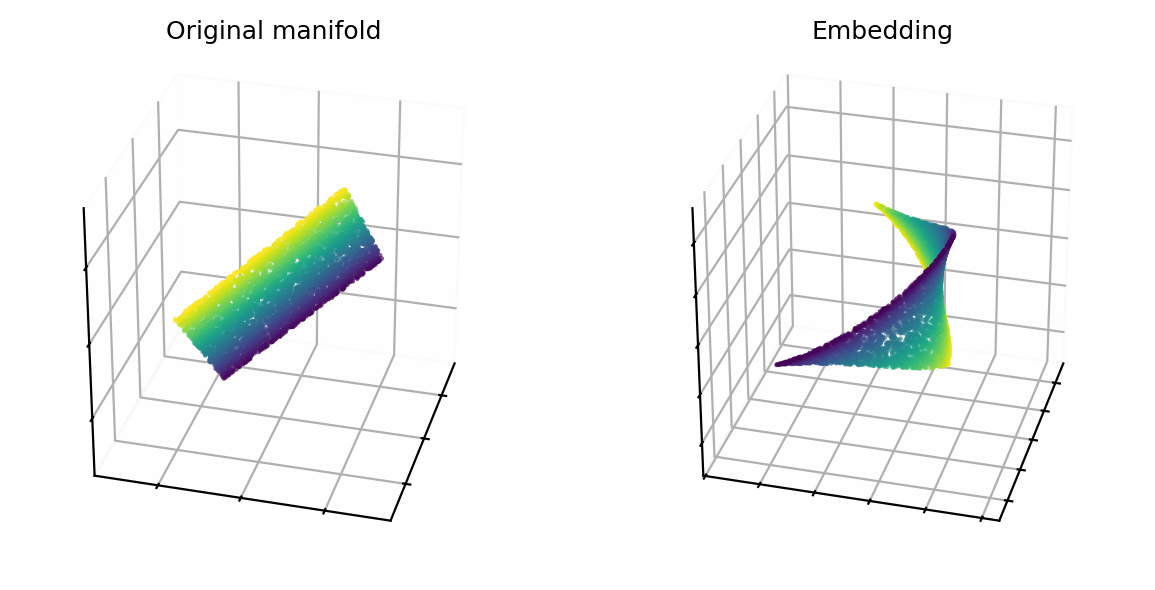
\includegraphics[width=0.8\textwidth]{figures/horseshoe.png}
  \caption{Diffusion maps on a bounded flat manifold exhibit the horseshoe phenomenon. Left: samples from a 2D linear subspace in $\R^3$. Right: the 3D diffusion-map embedding $(\phi_1,\phi_2,\phi_3)$, which bends the flat square into a horseshoe shape rather than recovering the plane.}
  \label{fig:horseshoe}
\end{figure}

\subsection{Experiments about $n$}
Our main theorems are for a family of manifolds, where the geometric quantities are defined independently of any sampling. In practice, a finite point cloud is used and it is only a numerical discretization of such a continuous object. The purpose of this experiment is to show that our estimates exhibit a convergence behavior: as the number of samples $n$ increases, the estimation error decreases steadily toward zero. Such convergence indicates that the estimated quantities genuinely approximate the underlying geometric quantities, which makes the measurements reported in our main experiments meaningful.

We illustrate this on two quantities. For the Riemannian metric, we sample $n$ points from the unit sphere $S^2$ and report the deviation of the estimated metric's singular values $\sigma$ from $1$, measured both on average ($\mathrm{mean}\,|\sigma-1|$) and in the worst case ($\max\,|\sigma-1|$). For the reach, we sample $n$ points from a torus with reach $\tau = 1.5$ and compare the estimate $\hat{\tau}$ against this ground truth. We vary $n \in \{500, 1000, 2000, 5000, 10000\}$, repeat each setting three times, and report the mean together with the min--max range.

\begin{figure}[htbp]
    \centering
    \begin{minipage}[t]{0.48\linewidth}
        \centering
        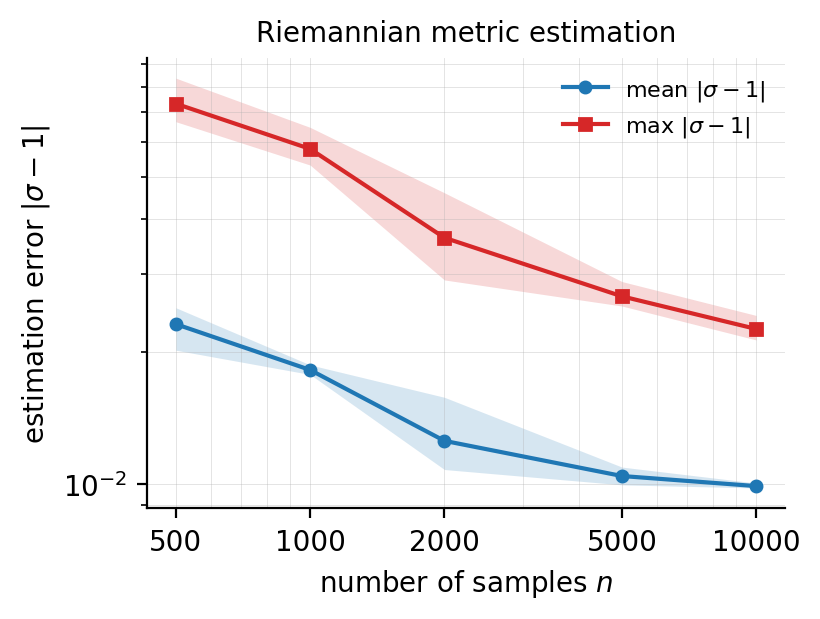
\includegraphics[width=\linewidth]{figures/rmetric.png}
        \caption{Metric estimation error on $S^2$ decreases as $n$ grows}
        \label{fig:metric}
    \end{minipage}%
    \hfill 
    \begin{minipage}[t]{0.48\linewidth}
        \centering
        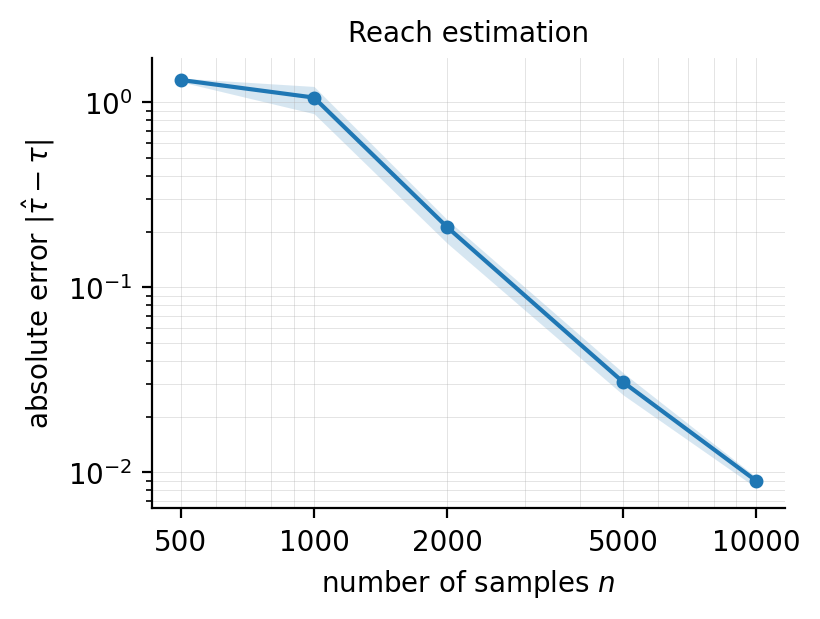
\includegraphics[width=\linewidth]{figures/reach.png}
        \caption{Reach estimation error on a torus ($\tau=1.5$) decreases as $n$ grows.}
        \label{fig:reach}
    \end{minipage}
    \label{fig:total}
\end{figure}

As shown in Figure~\ref{fig:metric} and Figure~\ref{fig:reach}, the estimation error decreases steadily as $n$ grows for both the Riemannian metric and the reach. This convergence confirms that our estimators are consistent in practice and that the measurements reported in our main experiments are meaningful.


\newpage
\section*{NeurIPS Paper Checklist}

%%% BEGIN INSTRUCTIONS %%%

%%% END INSTRUCTIONS %%%


\begin{enumerate}

\item {\bf Claims}
    \item[] Question: Do the main claims made in the abstract and introduction accurately reflect the paper's contributions and scope?
    \item[] Answer: \answerYes{} % Replace by \answerYes{}, \answerNo{}, or \answerNA{}.
    \item[] Justification: Yes. Abstract and Introduction include our claims.
    \item[] Guidelines:
    \begin{itemize}
        \item The answer \answerNA{} means that the abstract and introduction do not include the claims made in the paper.
        \item The abstract and/or introduction should clearly state the claims made, including the contributions made in the paper and important assumptions and limitations. A \answerNo{} or \answerNA{} answer to this question will not be perceived well by the reviewers. 
        \item The claims made should match theoretical and experimental results, and reflect how much the results can be expected to generalize to other settings. 
        \item It is fine to include aspirational goals as motivation as long as it is clear that these goals are not attained by the paper. 
    \end{itemize}

\item {\bf Limitations}
    \item[] Question: Does the paper discuss the limitations of the work performed by the authors?
    \item[] Answer: \answerYes{} % Replace by \answerYes{}, \answerNo{}, or \answerNA{}.
    \item[] Justification: Yes. We discussed the limitation of our work in the Conclusion section. 
	
	 Our regularity condition is very rigorous, to avoid embedding manifolds through DM having vanishing global reach. We have verified inequality related to this assumption along with all the other assumption holds for some well-behaved manifolds (see \cref{sec:S2}), but it is strict. 
	 
	 This paper includes only a few experiments for the following reasons:
        \begin{enumerate}
        \item  People do not have any method to compute eigenvalues and eigenfunctions for general manifolds, thus it is difficult or even impossible to derive the true tangent space and compute the estimating error.
        \item Our algorithm is designed for a family of manifolds $\mathcal{M}$ whose cardinality equals that of the continuum and whose members can vary drastically in their geometric structures. As a result, it is not feasible to conduct experiments over all possible manifolds, nor to reliably evaluate the algorithm based on a finite collection of representative manifolds.
        \item The constants involved in our theorem are merely asserted to exist and are not given in an explicit form. It is difficult to derive them through numerical simulations and then perform experiments.
        \end{enumerate}

    \item[] Guidelines:
    \begin{itemize}
        \item The answer \answerNA{} means that the paper has no limitation while the answer \answerNo{} means that the paper has limitations, but those are not discussed in the paper. 
        \item The authors are encouraged to create a separate ``Limitations'' section in their paper.
        \item The paper should point out any strong assumptions and how robust the results are to violations of these assumptions (e.g., independence assumptions, noiseless settings, model well-specification, asymptotic approximations only holding locally). The authors should reflect on how these assumptions might be violated in practice and what the implications would be.
        \item The authors should reflect on the scope of the claims made, e.g., if the approach was only tested on a few datasets or with a few runs. In general, empirical results often depend on implicit assumptions, which should be articulated.
        \item The authors should reflect on the factors that influence the performance of the approach. For example, a facial recognition algorithm may perform poorly when image resolution is low or images are taken in low lighting. Or a speech-to-text system might not be used reliably to provide closed captions for online lectures because it fails to handle technical jargon.
        \item The authors should discuss the computational efficiency of the proposed algorithms and how they scale with dataset size.
        \item If applicable, the authors should discuss possible limitations of their approach to address problems of privacy and fairness.
        \item While the authors might fear that complete honesty about limitations might be used by reviewers as grounds for rejection, a worse outcome might be that reviewers discover limitations that aren't acknowledged in the paper. The authors should use their best judgment and recognize that individual actions in favor of transparency play an important role in developing norms that preserve the integrity of the community. Reviewers will be specifically instructed to not penalize honesty concerning limitations.
    \end{itemize}

\item {\bf Theory assumptions and proofs}
    \item[] Question: For each theoretical result, does the paper provide the full set of assumptions and a complete (and correct) proof?
    \item[] Answer: \answerYes{} % Replace by \answerYes{}, \answerNo{}, or \answerNA{}.
    \item[] Justification: Yes. We list all assumptions in \cref{sec:problem}. For theorem in main part, see \cref{sec:phiM-summary} and \cref{phiM}. For lemma and theorem in appendix, we show proof or give reference.
    \item[] Guidelines:
    \begin{itemize}
        \item The answer \answerNA{} means that the paper does not include theoretical results. 
        \item All the theorems, formulas, and proofs in the paper should be numbered and cross-referenced.
        \item All assumptions should be clearly stated or referenced in the statement of any theorems.
        \item The proofs can either appear in the main paper or the supplemental material, but if they appear in the supplemental material, the authors are encouraged to provide a short proof sketch to provide intuition. 
        \item Inversely, any informal proof provided in the core of the paper should be complemented by formal proofs provided in appendix or supplemental material.
        \item Theorems and Lemmas that the proof relies upon should be properly referenced. 
    \end{itemize}

    \item {\bf Experimental result reproducibility}
    \item[] Question: Does the paper fully disclose all the information needed to reproduce the main experimental results of the paper to the extent that it affects the main claims and/or conclusions of the paper (regardless of whether the code and data are provided or not)?
    \item[] Answer: \answerYes{} % Replace by \answerYes{}, \answerNo{}, or \answerNA{}.
    \item[] Justification: Yes. We provide all algorithm needed and their references to reproduce experiments. We also provide code and parameters in the supplemental material.
    \item[] Guidelines:
    \begin{itemize}
        \item The answer \answerNA{} means that the paper does not include experiments.
        \item If the paper includes experiments, a \answerNo{} answer to this question will not be perceived well by the reviewers: Making the paper reproducible is important, regardless of whether the code and data are provided or not.
        \item If the contribution is a dataset and\slash or model, the authors should describe the steps taken to make their results reproducible or verifiable. 
        \item Depending on the contribution, reproducibility can be accomplished in various ways. For example, if the contribution is a novel architecture, describing the architecture fully might suffice, or if the contribution is a specific model and empirical evaluation, it may be necessary to either make it possible for others to replicate the model with the same dataset, or provide access to the model. In general. releasing code and data is often one good way to accomplish this, but reproducibility can also be provided via detailed instructions for how to replicate the results, access to a hosted model (e.g., in the case of a large language model), releasing of a model checkpoint, or other means that are appropriate to the research performed.
        \item While NeurIPS does not require releasing code, the conference does require all submissions to provide some reasonable avenue for reproducibility, which may depend on the nature of the contribution. For example
        \begin{enumerate}
            \item If the contribution is primarily a new algorithm, the paper should make it clear how to reproduce that algorithm.
            \item If the contribution is primarily a new model architecture, the paper should describe the architecture clearly and fully.
            \item If the contribution is a new model (e.g., a large language model), then there should either be a way to access this model for reproducing the results or a way to reproduce the model (e.g., with an open-source dataset or instructions for how to construct the dataset).
            \item We recognize that reproducibility may be tricky in some cases, in which case authors are welcome to describe the particular way they provide for reproducibility. In the case of closed-source models, it may be that access to the model is limited in some way (e.g., to registered users), but it should be possible for other researchers to have some path to reproducing or verifying the results.
        \end{enumerate}
    \end{itemize}


\item {\bf Open access to data and code}
    \item[] Question: Does the paper provide open access to the data and code, with sufficient instructions to faithfully reproduce the main experimental results, as described in supplemental material?
    \item[] Answer: \answerYes{} % Replace by \answerYes{}, \answerNo{}, or \answerNA{}.
    \item[] Justification: Yes. We provide code and parameters in the supplemental material.
    \item[] Guidelines:
    \begin{itemize}
        \item The answer \answerNA{} means that paper does not include experiments requiring code.
        \item Please see the NeurIPS code and data submission guidelines (\url{https://neurips.cc/public/guides/CodeSubmissionPolicy}) for more details.
        \item While we encourage the release of code and data, we understand that this might not be possible, so \answerNo{} is an acceptable answer. Papers cannot be rejected simply for not including code, unless this is central to the contribution (e.g., for a new open-source benchmark).
        \item The instructions should contain the exact command and environment needed to run to reproduce the results. See the NeurIPS code and data submission guidelines (\url{https://neurips.cc/public/guides/CodeSubmissionPolicy}) for more details.
        \item The authors should provide instructions on data access and preparation, including how to access the raw data, preprocessed data, intermediate data, and generated data, etc.
        \item The authors should provide scripts to reproduce all experimental results for the new proposed method and baselines. If only a subset of experiments are reproducible, they should state which ones are omitted from the script and why.
        \item At submission time, to preserve anonymity, the authors should release anonymized versions (if applicable).
        \item Providing as much information as possible in supplemental material (appended to the paper) is recommended, but including URLs to data and code is permitted.
    \end{itemize}


\item {\bf Experimental setting/details}
    \item[] Question: Does the paper specify all the training and test details (e.g., data splits, hyperparameters, how they were chosen, type of optimizer) necessary to understand the results?
    \item[] Answer: \answerYes{} % Replace by \answerYes{}, \answerNo{}, or \answerNA{}.
    \item[] Justification: We specify the generating process and we only have very few parameters to choose, so grid search is used. 
    \item[] Guidelines:
    \begin{itemize}
        \item The answer \answerNA{} means that the paper does not include experiments.
        \item The experimental setting should be presented in the core of the paper to a level of detail that is necessary to appreciate the results and make sense of them.
        \item The full details can be provided either with the code, in appendix, or as supplemental material.
    \end{itemize}

\item {\bf Experiment statistical significance}
    \item[] Question: Does the paper report error bars suitably and correctly defined or other appropriate information about the statistical significance of the experiments?
    \item[] Answer: \answerNo{} % Replace by \answerYes{}, \answerNo{}, or \answerNA{}.
    \item[] Justification: In the manifold learning setting, the estimation error is not Gaussian and the error bar is not well defined. Besides, large sample size vanishes the variance of the estimation error, which is the case of this paper.
    \item[] Guidelines:
    \begin{itemize}
        \item The answer \answerNA{} means that the paper does not include experiments.
        \item The authors should answer \answerYes{} if the results are accompanied by error bars, confidence intervals, or statistical significance tests, at least for the experiments that support the main claims of the paper.
        \item The factors of variability that the error bars are capturing should be clearly stated (for example, train/test split, initialization, random drawing of some parameter, or overall run with given experimental conditions).
        \item The method for calculating the error bars should be explained (closed form formula, call to a library function, bootstrap, etc.)
        \item The assumptions made should be given (e.g., Normally distributed errors).
        \item It should be clear whether the error bar is the standard deviation or the standard error of the mean.
        \item It is OK to report 1-sigma error bars, but one should state it. The authors should preferably report a 2-sigma error bar than state that they have a 96\% CI, if the hypothesis of Normality of errors is not verified.
        \item For asymmetric distributions, the authors should be careful not to show in tables or figures symmetric error bars that would yield results that are out of range (e.g., negative error rates).
        \item If error bars are reported in tables or plots, the authors should explain in the text how they were calculated and reference the corresponding figures or tables in the text.
    \end{itemize}

\item {\bf Experiments compute resources}
    \item[] Question: For each experiment, does the paper provide sufficient information on the computer resources (type of compute workers, memory, time of execution) needed to reproduce the experiments?
    \item[] Answer: \answerYes{} % Replace by \answerYes{}, \answerNo{}, or \answerNA{}.
    \item[] Justification: We specify the experimental platform and running time in Experiment section.
    \item[] Guidelines:
    \begin{itemize}
        \item The answer \answerNA{} means that the paper does not include experiments.
        \item The paper should indicate the type of compute workers CPU or GPU, internal cluster, or cloud provider, including relevant memory and storage.
        \item The paper should provide the amount of compute required for each of the individual experimental runs as well as estimate the total compute. 
        \item The paper should disclose whether the full research project required more compute than the experiments reported in the paper (e.g., preliminary or failed experiments that didn't make it into the paper). 
    \end{itemize}
    
\item {\bf Code of ethics}
    \item[] Question: Does the research conducted in the paper conform, in every respect, with the NeurIPS Code of Ethics \url{https://neurips.cc/public/EthicsGuidelines}?
    \item[] Answer: \answerYes{} % Replace by \answerYes{}, \answerNo{}, or \answerNA{}.
    \item[] Justification: We followed the NeurIPS Code of Ethics.
    \item[] Guidelines:
    \begin{itemize}
        \item The answer \answerNA{} means that the authors have not reviewed the NeurIPS Code of Ethics.
        \item If the authors answer \answerNo, they should explain the special circumstances that require a deviation from the Code of Ethics.
        \item The authors should make sure to preserve anonymity (e.g., if there is a special consideration due to laws or regulations in their jurisdiction).
    \end{itemize}


\item {\bf Broader impacts}
    \item[] Question: Does the paper discuss both potential positive societal impacts and negative societal impacts of the work performed?
    \item[] Answer: \answerNA{} % Replace by \answerYes{}, \answerNo{}, or \answerNA{}.
    \item[] Justification: This research is not tied to particular applications and to our knowledge there are no direct paths to negative applications.  
    \item[] Guidelines:
    \begin{itemize}
        \item The answer \answerNA{} means that there is no societal impact of the work performed.
        \item If the authors answer \answerNA{} or \answerNo, they should explain why their work has no societal impact or why the paper does not address societal impact.
        \item Examples of negative societal impacts include potential malicious or unintended uses (e.g., disinformation, generating fake profiles, surveillance), fairness considerations (e.g., deployment of technologies that could make decisions that unfairly impact specific groups), privacy considerations, and security considerations.
        \item The conference expects that many papers will be foundational research and not tied to particular applications, let alone deployments. However, if there is a direct path to any negative applications, the authors should point it out. For example, it is legitimate to point out that an improvement in the quality of generative models could be used to generate Deepfakes for disinformation. On the other hand, it is not needed to point out that a generic algorithm for optimizing neural networks could enable people to train models that generate Deepfakes faster.
        \item The authors should consider possible harms that could arise when the technology is being used as intended and functioning correctly, harms that could arise when the technology is being used as intended but gives incorrect results, and harms following from (intentional or unintentional) misuse of the technology.
        \item If there are negative societal impacts, the authors could also discuss possible mitigation strategies (e.g., gated release of models, providing defenses in addition to attacks, mechanisms for monitoring misuse, mechanisms to monitor how a system learns from feedback over time, improving the efficiency and accessibility of ML).
    \end{itemize}
    
\item {\bf Safeguards}
    \item[] Question: Does the paper describe safeguards that have been put in place for responsible release of data or models that have a high risk for misuse (e.g., pre-trained language models, image generators, or scraped datasets)?
    \item[] Answer: \answerNA{} % Replace by \answerYes{}, \answerNo{}, or \answerNA{}.
    \item[] Justification: The paper poses no safeguards risks.
    \item[] Guidelines:
    \begin{itemize}
        \item The answer \answerNA{} means that the paper poses no such risks.
        \item Released models that have a high risk for misuse or dual-use should be released with necessary safeguards to allow for controlled use of the model, for example by requiring that users adhere to usage guidelines or restrictions to access the model or implementing safety filters. 
        \item Datasets that have been scraped from the Internet could pose safety risks. The authors should describe how they avoided releasing unsafe images.
        \item We recognize that providing effective safeguards is challenging, and many papers do not require this, but we encourage authors to take this into account and make a best faith effort.
    \end{itemize}

\item {\bf Licenses for existing assets}
    \item[] Question: Are the creators or original owners of assets (e.g., code, data, models), used in the paper, properly credited and are the license and terms of use explicitly mentioned and properly respected?
    \item[] Answer: \answerNA{} % Replace by \answerYes{}, \answerNo{}, or \answerNA{}.
    \item[] Justification: The paper does not use existing assets.
    \item[] Guidelines:
    \begin{itemize}
        \item The answer \answerNA{} means that the paper does not use existing assets.
        \item The authors should cite the original paper that produced the code package or dataset.
        \item The authors should state which version of the asset is used and, if possible, include a URL.
        \item The name of the license (e.g., CC-BY 4.0) should be included for each asset.
        \item For scraped data from a particular source (e.g., website), the copyright and terms of service of that source should be provided.
        \item If assets are released, the license, copyright information, and terms of use in the package should be provided. For popular datasets, \url{paperswithcode.com/datasets} has curated licenses for some datasets. Their licensing guide can help determine the license of a dataset.
        \item For existing datasets that are re-packaged, both the original license and the license of the derived asset (if it has changed) should be provided.
        \item If this information is not available online, the authors are encouraged to reach out to the asset's creators.
    \end{itemize}

\item {\bf New assets}
    \item[] Question: Are new assets introduced in the paper well documented and is the documentation provided alongside the assets?
    \item[] Answer: \answerNA{} % Replace by \answerYes{}, \answerNo{}, or \answerNA{}.
    \item[] Justification: The paper does not release new assets.
    \item[] Guidelines:
    \begin{itemize}
        \item The answer \answerNA{} means that the paper does not release new assets.
        \item Researchers should communicate the details of the dataset\slash code\slash model as part of their submissions via structured templates. This includes details about training, license, limitations, etc. 
        \item The paper should discuss whether and how consent was obtained from people whose asset is used.
        \item At submission time, remember to anonymize your assets (if applicable). You can either create an anonymized URL or include an anonymized zip file.
    \end{itemize}

\item {\bf Crowdsourcing and research with human subjects}
    \item[] Question: For crowdsourcing experiments and research with human subjects, does the paper include the full text of instructions given to participants and screenshots, if applicable, as well as details about compensation (if any)? 
    \item[] Answer: \answerNA{} % Replace by \answerYes{}, \answerNo{}, or \answerNA{}.
    \item[] Justification: The paper does not involve crowdsourcing nor research with human subjects.
    \item[] Guidelines:
    \begin{itemize}
        \item The answer \answerNA{} means that the paper does not involve crowdsourcing nor research with human subjects.
        \item Including this information in the supplemental material is fine, but if the main contribution of the paper involves human subjects, then as much detail as possible should be included in the main paper. 
        \item According to the NeurIPS Code of Ethics, workers involved in data collection, curation, or other labor should be paid at least the minimum wage in the country of the data collector. 
    \end{itemize}

\item {\bf Institutional review board (IRB) approvals or equivalent for research with human subjects}
    \item[] Question: Does the paper describe potential risks incurred by study participants, whether such risks were disclosed to the subjects, and whether Institutional Review Board (IRB) approvals (or an equivalent approval/review based on the requirements of your country or institution) were obtained?
    \item[] Answer: \answerNA{} % Replace by \answerYes{}, \answerNo{}, or \answerNA{}.
    \item[] Justification: The paper does not involve crowdsourcing nor research with human subjects.
    \item[] Guidelines:
    \begin{itemize}
        \item The answer \answerNA{} means that the paper does not involve crowdsourcing nor research with human subjects.
        \item Depending on the country in which research is conducted, IRB approval (or equivalent) may be required for any human subjects research. If you obtained IRB approval, you should clearly state this in the paper. 
        \item We recognize that the procedures for this may vary significantly between institutions and locations, and we expect authors to adhere to the NeurIPS Code of Ethics and the guidelines for their institution. 
        \item For initial submissions, do not include any information that would break anonymity (if applicable), such as the institution conducting the review.
    \end{itemize}

\item {\bf Declaration of LLM usage}
    \item[] Question: Does the paper describe the usage of LLMs if it is an important, original, or non-standard component of the core methods in this research? Note that if the LLM is used only for writing, editing, or formatting purposes and does \emph{not} impact the core methodology, scientific rigor, or originality of the research, declaration is not required.
    %this research? 
    \item[] Answer: \answerNA{} % Replace by \answerYes{}, \answerNo{}, or \answerNA{}.
    \item[] Justification: The core method development in this research does not involve LLMs as any important, original, or non-standard components.
    \item[] Guidelines:
    \begin{itemize}
        \item The answer \answerNA{} means that the core method development in this research does not involve LLMs as any important, original, or non-standard components.
        \item Please refer to our LLM policy in the NeurIPS handbook for what should or should not be described.
    \end{itemize}

\end{enumerate}
\end{document}
***********************************
